\documentclass[twoside]{book}

% Packages required by doxygen
\usepackage{fixltx2e}
\usepackage{calc}
\usepackage{doxygen}
\usepackage[export]{adjustbox} % also loads graphicx
\usepackage{graphicx}
\usepackage[utf8]{inputenc}
\usepackage{makeidx}
\usepackage{multicol}
\usepackage{multirow}
\PassOptionsToPackage{warn}{textcomp}
\usepackage{textcomp}
\usepackage[nointegrals]{wasysym}
\usepackage[table]{xcolor}

% Font selection
\usepackage[T1]{fontenc}
\usepackage[scaled=.90]{helvet}
\usepackage{courier}
\usepackage{amssymb}
\usepackage{sectsty}
\renewcommand{\familydefault}{\sfdefault}
\allsectionsfont{%
  \fontseries{bc}\selectfont%
  \color{darkgray}%
}
\renewcommand{\DoxyLabelFont}{%
  \fontseries{bc}\selectfont%
  \color{darkgray}%
}
\newcommand{\+}{\discretionary{\mbox{\scriptsize$\hookleftarrow$}}{}{}}

% Page & text layout
\usepackage{geometry}
\geometry{%
  a4paper,%
  top=2.5cm,%
  bottom=2.5cm,%
  left=2.5cm,%
  right=2.5cm%
}
\tolerance=750
\hfuzz=15pt
\hbadness=750
\setlength{\emergencystretch}{15pt}
\setlength{\parindent}{0cm}
\setlength{\parskip}{3ex plus 2ex minus 2ex}
\makeatletter
\renewcommand{\paragraph}{%
  \@startsection{paragraph}{4}{0ex}{-1.0ex}{1.0ex}{%
    \normalfont\normalsize\bfseries\SS@parafont%
  }%
}
\renewcommand{\subparagraph}{%
  \@startsection{subparagraph}{5}{0ex}{-1.0ex}{1.0ex}{%
    \normalfont\normalsize\bfseries\SS@subparafont%
  }%
}
\makeatother

% Headers & footers
\usepackage{fancyhdr}
\pagestyle{fancyplain}
\fancyhead[LE]{\fancyplain{}{\bfseries\thepage}}
\fancyhead[CE]{\fancyplain{}{}}
\fancyhead[RE]{\fancyplain{}{\bfseries\leftmark}}
\fancyhead[LO]{\fancyplain{}{\bfseries\rightmark}}
\fancyhead[CO]{\fancyplain{}{}}
\fancyhead[RO]{\fancyplain{}{\bfseries\thepage}}
\fancyfoot[LE]{\fancyplain{}{}}
\fancyfoot[CE]{\fancyplain{}{}}
\fancyfoot[RE]{\fancyplain{}{\bfseries\scriptsize Generated by Doxygen }}
\fancyfoot[LO]{\fancyplain{}{\bfseries\scriptsize Generated by Doxygen }}
\fancyfoot[CO]{\fancyplain{}{}}
\fancyfoot[RO]{\fancyplain{}{}}
\renewcommand{\footrulewidth}{0.4pt}
\renewcommand{\chaptermark}[1]{%
  \markboth{#1}{}%
}
\renewcommand{\sectionmark}[1]{%
  \markright{\thesection\ #1}%
}

% Indices & bibliography
\usepackage{natbib}
\usepackage[titles]{tocloft}
\setcounter{tocdepth}{3}
\setcounter{secnumdepth}{5}
\makeindex

% Hyperlinks (required, but should be loaded last)
\usepackage{ifpdf}
\ifpdf
  \usepackage[pdftex,pagebackref=true]{hyperref}
\else
  \usepackage[ps2pdf,pagebackref=true]{hyperref}
\fi
\hypersetup{%
  colorlinks=true,%
  linkcolor=blue,%
  citecolor=blue,%
  unicode%
}

% Custom commands
\newcommand{\clearemptydoublepage}{%
  \newpage{\pagestyle{empty}\cleardoublepage}%
}

\usepackage{caption}
\captionsetup{labelsep=space,justification=centering,font={bf},singlelinecheck=off,skip=4pt,position=top}

%===== C O N T E N T S =====

\begin{document}

% Titlepage & ToC
\hypersetup{pageanchor=false,
             bookmarksnumbered=true,
             pdfencoding=unicode
            }
\pagenumbering{alph}
\begin{titlepage}
\vspace*{7cm}
\begin{center}%
{\Large Adaptive\+Dummy\+Process \\[1ex]\large 1 }\\
\vspace*{1cm}
{\large Generated by Doxygen 1.8.13}\\
\end{center}
\end{titlepage}
\clearemptydoublepage
\pagenumbering{roman}
\tableofcontents
\clearemptydoublepage
\pagenumbering{arabic}
\hypersetup{pageanchor=true}

%--- Begin generated contents ---
\chapter{Class Index}
\section{Class List}
Here are the classes, structs, unions and interfaces with brief descriptions\+:\begin{DoxyCompactList}
\item\contentsline{section}{\hyperlink{classchecksum__manager}{checksum\+\_\+manager} \\*Class of checksum manager for \hyperlink{structCRC}{C\+RC} managment }{\pageref{classchecksum__manager}}{}
\item\contentsline{section}{\hyperlink{structCRC}{C\+RC} }{\pageref{structCRC}}{}
\item\contentsline{section}{\hyperlink{classdeserializer}{deserializer} \\*Class of deserializer which handles deserialization of data from files and shared memory }{\pageref{classdeserializer}}{}
\item\contentsline{section}{\hyperlink{structEXMPLE__s}{E\+X\+M\+P\+L\+E\+\_\+s} }{\pageref{structEXMPLE__s}}{}
\item\contentsline{section}{\hyperlink{classmessage__manager}{message\+\_\+manager} \\*Class of message manager which handles the synchronization between processes }{\pageref{classmessage__manager}}{}
\item\contentsline{section}{\hyperlink{classshared__memory}{shared\+\_\+memory} }{\pageref{classshared__memory}}{}
\item\contentsline{section}{\hyperlink{structUMGR__s}{U\+M\+G\+R\+\_\+s} \\*Struct which is specified to hold the values of the Update\+Manager U\+M\+GR }{\pageref{structUMGR__s}}{}
\end{DoxyCompactList}

\chapter{File Index}
\section{File List}
Here is a list of all files with brief descriptions\+:\begin{DoxyCompactList}
\item\contentsline{section}{/home/visxim/\+C\+Lion\+Projects/\+Adaptive\+Dummy\+Process/\hyperlink{checksum__manager_8cpp}{checksum\+\_\+manager.\+cpp} \\*Checksum\+\_\+manager for checking the integrity of the data }{\pageref{checksum__manager_8cpp}}{}
\item\contentsline{section}{/home/visxim/\+C\+Lion\+Projects/\+Adaptive\+Dummy\+Process/\hyperlink{deserializer_8cpp}{deserializer.\+cpp} \\*Deserializer for deserializing the parsed configuration data }{\pageref{deserializer_8cpp}}{}
\item\contentsline{section}{/home/visxim/\+C\+Lion\+Projects/\+Adaptive\+Dummy\+Process/\hyperlink{main_8cpp}{main.\+cpp} \\*Main of the Adaptive\+Dummy\+Process }{\pageref{main_8cpp}}{}
\item\contentsline{section}{/home/visxim/\+C\+Lion\+Projects/\+Adaptive\+Dummy\+Process/\hyperlink{message__manager_8cpp}{message\+\_\+manager.\+cpp} \\*Message\+\_\+manager for managing the synchronization between processes }{\pageref{message__manager_8cpp}}{}
\item\contentsline{section}{/home/visxim/\+C\+Lion\+Projects/\+Adaptive\+Dummy\+Process/\hyperlink{shared__memory_8cpp}{shared\+\_\+memory.\+cpp} }{\pageref{shared__memory_8cpp}}{}
\item\contentsline{section}{/home/visxim/\+C\+Lion\+Projects/\+Adaptive\+Dummy\+Process/\hyperlink{time-tp_8cpp}{time-\/tp.\+cpp} }{\pageref{time-tp_8cpp}}{}
\item\contentsline{section}{/home/visxim/\+C\+Lion\+Projects/\+Adaptive\+Dummy\+Process/includes/\hyperlink{checksum__manager_8h}{checksum\+\_\+manager.\+h} \\*Header of \hyperlink{classchecksum__manager}{checksum\+\_\+manager} for checking the integrity of the data }{\pageref{checksum__manager_8h}}{}
\item\contentsline{section}{/home/visxim/\+C\+Lion\+Projects/\+Adaptive\+Dummy\+Process/includes/\hyperlink{data__storage_8h}{data\+\_\+storage.\+h} \\*Header of \hyperlink{classchecksum__manager}{checksum\+\_\+manager} for checking the integrity of the data }{\pageref{data__storage_8h}}{}
\item\contentsline{section}{/home/visxim/\+C\+Lion\+Projects/\+Adaptive\+Dummy\+Process/includes/\hyperlink{deserializer_8h}{deserializer.\+h} \\*Header of deserializer for deserializing the parsed configuration data }{\pageref{deserializer_8h}}{}
\item\contentsline{section}{/home/visxim/\+C\+Lion\+Projects/\+Adaptive\+Dummy\+Process/includes/\hyperlink{message__manager_8h}{message\+\_\+manager.\+h} \\*Header of \hyperlink{classmessage__manager}{message\+\_\+manager} for managing the synchronization between processes }{\pageref{message__manager_8h}}{}
\item\contentsline{section}{/home/visxim/\+C\+Lion\+Projects/\+Adaptive\+Dummy\+Process/includes/\hyperlink{shared__memory_8h}{shared\+\_\+memory.\+h} }{\pageref{shared__memory_8h}}{}
\item\contentsline{section}{/home/visxim/\+C\+Lion\+Projects/\+Adaptive\+Dummy\+Process/includes/\hyperlink{time-tp_8h}{time-\/tp.\+h} }{\pageref{time-tp_8h}}{}
\end{DoxyCompactList}

\chapter{Class Documentation}
\hypertarget{classchecksum__manager}{}\section{checksum\+\_\+manager Class Reference}
\label{classchecksum__manager}\index{checksum\+\_\+manager@{checksum\+\_\+manager}}


Class of checksum manager for \hyperlink{structCRC}{C\+RC} managment.  




{\ttfamily \#include $<$checksum\+\_\+manager.\+h$>$}

\subsection*{Public Member Functions}
\begin{DoxyCompactItemize}
\item 
int \hyperlink{classchecksum__manager_a31afd631fa3668a1dfd08ee0b8807d16}{create\+C\+RC} (\hyperlink{structUMGR__s}{U\+M\+G\+R\+\_\+s} $\ast$C\+R\+Cdata)
\begin{DoxyCompactList}\small\item\em This method is overloaded for every struct in data\+\_\+storage. \end{DoxyCompactList}\item 
int \hyperlink{classchecksum__manager_a613cc124da07b2f7d002eefb2065a2e3}{create\+C\+RC} (\hyperlink{structEXMPLE__s}{E\+X\+M\+P\+L\+E\+\_\+s} $\ast$C\+R\+Cdata)
\begin{DoxyCompactList}\small\item\em Function for creating the checksum. \end{DoxyCompactList}\item 
int \hyperlink{classchecksum__manager_a14eeba6bf4d2ad333c227339bd453a72}{check\+C\+RC} (\hyperlink{structUMGR__s}{U\+M\+G\+R\+\_\+s} $\ast$C\+R\+Cdata)
\begin{DoxyCompactList}\small\item\em Function for checking the checksum. \end{DoxyCompactList}\item 
int \hyperlink{classchecksum__manager_a74f8d881aee7981cc60b2d169915bc4e}{check\+C\+RC} (\hyperlink{structEXMPLE__s}{E\+X\+M\+P\+L\+E\+\_\+s} $\ast$C\+R\+Cdata)
\begin{DoxyCompactList}\small\item\em Function for checking the checksum. \end{DoxyCompactList}\end{DoxyCompactItemize}


\subsection{Detailed Description}
Class of checksum manager for \hyperlink{structCRC}{C\+RC} managment. 

\subsection{Member Function Documentation}
\mbox{\Hypertarget{classchecksum__manager_a14eeba6bf4d2ad333c227339bd453a72}\label{classchecksum__manager_a14eeba6bf4d2ad333c227339bd453a72}} 
\index{checksum\+\_\+manager@{checksum\+\_\+manager}!check\+C\+RC@{check\+C\+RC}}
\index{check\+C\+RC@{check\+C\+RC}!checksum\+\_\+manager@{checksum\+\_\+manager}}
\subsubsection{\texorpdfstring{check\+C\+R\+C()}{checkCRC()}\hspace{0.1cm}{\footnotesize\ttfamily [1/2]}}
{\footnotesize\ttfamily int checksum\+\_\+manager\+::check\+C\+RC (\begin{DoxyParamCaption}\item[{\hyperlink{structUMGR__s}{U\+M\+G\+R\+\_\+s} $\ast$}]{C\+R\+Cdata }\end{DoxyParamCaption})}



Function for checking the checksum. 

Needs to be overloaded for different data structures Compare the received checksum with the self calculated Here is the call graph for this function\+:
\nopagebreak
\begin{figure}[H]
\begin{center}
\leavevmode
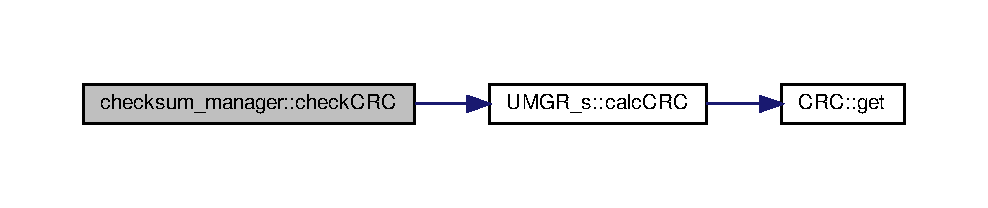
\includegraphics[width=350pt]{classchecksum__manager_a14eeba6bf4d2ad333c227339bd453a72_cgraph}
\end{center}
\end{figure}
\mbox{\Hypertarget{classchecksum__manager_a74f8d881aee7981cc60b2d169915bc4e}\label{classchecksum__manager_a74f8d881aee7981cc60b2d169915bc4e}} 
\index{checksum\+\_\+manager@{checksum\+\_\+manager}!check\+C\+RC@{check\+C\+RC}}
\index{check\+C\+RC@{check\+C\+RC}!checksum\+\_\+manager@{checksum\+\_\+manager}}
\subsubsection{\texorpdfstring{check\+C\+R\+C()}{checkCRC()}\hspace{0.1cm}{\footnotesize\ttfamily [2/2]}}
{\footnotesize\ttfamily int checksum\+\_\+manager\+::check\+C\+RC (\begin{DoxyParamCaption}\item[{\hyperlink{structEXMPLE__s}{E\+X\+M\+P\+L\+E\+\_\+s} $\ast$}]{C\+R\+Cdata }\end{DoxyParamCaption})}



Function for checking the checksum. 

Needs to be overloaded for different data structures Process all bytes of the struct

Compare the received checksum with the self calculated \mbox{\Hypertarget{classchecksum__manager_a31afd631fa3668a1dfd08ee0b8807d16}\label{classchecksum__manager_a31afd631fa3668a1dfd08ee0b8807d16}} 
\index{checksum\+\_\+manager@{checksum\+\_\+manager}!create\+C\+RC@{create\+C\+RC}}
\index{create\+C\+RC@{create\+C\+RC}!checksum\+\_\+manager@{checksum\+\_\+manager}}
\subsubsection{\texorpdfstring{create\+C\+R\+C()}{createCRC()}\hspace{0.1cm}{\footnotesize\ttfamily [1/2]}}
{\footnotesize\ttfamily int checksum\+\_\+manager\+::create\+C\+RC (\begin{DoxyParamCaption}\item[{\hyperlink{structUMGR__s}{U\+M\+G\+R\+\_\+s} $\ast$}]{C\+R\+Cdata }\end{DoxyParamCaption})}



This method is overloaded for every struct in data\+\_\+storage. 

Function for creating the checksum.

Needs to be overloaded for different data structures Here is the call graph for this function\+:
\nopagebreak
\begin{figure}[H]
\begin{center}
\leavevmode
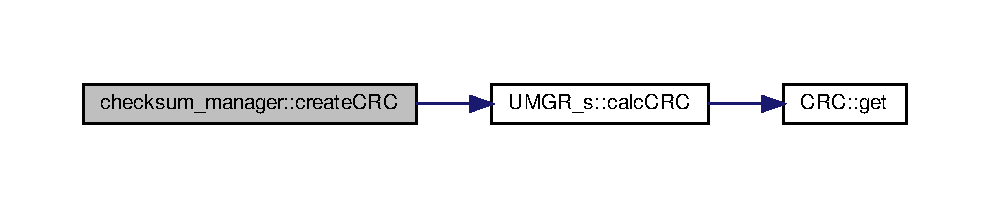
\includegraphics[width=350pt]{classchecksum__manager_a31afd631fa3668a1dfd08ee0b8807d16_cgraph}
\end{center}
\end{figure}
\mbox{\Hypertarget{classchecksum__manager_a613cc124da07b2f7d002eefb2065a2e3}\label{classchecksum__manager_a613cc124da07b2f7d002eefb2065a2e3}} 
\index{checksum\+\_\+manager@{checksum\+\_\+manager}!create\+C\+RC@{create\+C\+RC}}
\index{create\+C\+RC@{create\+C\+RC}!checksum\+\_\+manager@{checksum\+\_\+manager}}
\subsubsection{\texorpdfstring{create\+C\+R\+C()}{createCRC()}\hspace{0.1cm}{\footnotesize\ttfamily [2/2]}}
{\footnotesize\ttfamily int checksum\+\_\+manager\+::create\+C\+RC (\begin{DoxyParamCaption}\item[{\hyperlink{structEXMPLE__s}{E\+X\+M\+P\+L\+E\+\_\+s} $\ast$}]{C\+R\+Cdata }\end{DoxyParamCaption})}



Function for creating the checksum. 

Needs to be overloaded for different data structures Process all bytes of the struct 

The documentation for this class was generated from the following files\+:\begin{DoxyCompactItemize}
\item 
/home/visxim/\+C\+Lion\+Projects/\+Adaptive\+Dummy\+Process/includes/\hyperlink{checksum__manager_8h}{checksum\+\_\+manager.\+h}\item 
/home/visxim/\+C\+Lion\+Projects/\+Adaptive\+Dummy\+Process/\hyperlink{checksum__manager_8cpp}{checksum\+\_\+manager.\+cpp}\end{DoxyCompactItemize}

\hypertarget{structCRC}{}\section{C\+RC Struct Reference}
\label{structCRC}\index{C\+RC@{C\+RC}}


{\ttfamily \#include $<$data\+\_\+storage.\+h$>$}

\subsection*{Public Member Functions}
\begin{DoxyCompactItemize}
\item 
void \hyperlink{structCRC_a8d02f69866f0cbae7e8b1a41bc9c2d5b}{operator()} (string\+\_\+view s)
\item 
{\footnotesize template$<$typename T , typename  = std\+::enable\+\_\+if\+\_\+t$<$is\+\_\+integral\+\_\+v$<$\+T$>$$>$$>$ }\\void \hyperlink{structCRC_a3a15630422ed9cdd975336ec7d350beb}{operator()} (T const \&i)
\item 
auto \hyperlink{structCRC_adc0b899f86ac85515fad84e749033c61}{get} ()
\end{DoxyCompactItemize}
\subsection*{Public Attributes}
\begin{DoxyCompactItemize}
\item 
boost\+::crc\+\_\+32\+\_\+type \hyperlink{structCRC_aff4391b2e5fbfad71138bed74eaf5b11}{crc}
\end{DoxyCompactItemize}


\subsection{Member Function Documentation}
\mbox{\Hypertarget{structCRC_adc0b899f86ac85515fad84e749033c61}\label{structCRC_adc0b899f86ac85515fad84e749033c61}} 
\index{C\+RC@{C\+RC}!get@{get}}
\index{get@{get}!C\+RC@{C\+RC}}
\subsubsection{\texorpdfstring{get()}{get()}}
{\footnotesize\ttfamily auto C\+R\+C\+::get (\begin{DoxyParamCaption}{ }\end{DoxyParamCaption})\hspace{0.3cm}{\ttfamily [inline]}}

\mbox{\Hypertarget{structCRC_a8d02f69866f0cbae7e8b1a41bc9c2d5b}\label{structCRC_a8d02f69866f0cbae7e8b1a41bc9c2d5b}} 
\index{C\+RC@{C\+RC}!operator()@{operator()}}
\index{operator()@{operator()}!C\+RC@{C\+RC}}
\subsubsection{\texorpdfstring{operator()()}{operator()()}\hspace{0.1cm}{\footnotesize\ttfamily [1/2]}}
{\footnotesize\ttfamily void C\+R\+C\+::operator() (\begin{DoxyParamCaption}\item[{string\+\_\+view}]{s }\end{DoxyParamCaption})\hspace{0.3cm}{\ttfamily [inline]}}

\mbox{\Hypertarget{structCRC_a3a15630422ed9cdd975336ec7d350beb}\label{structCRC_a3a15630422ed9cdd975336ec7d350beb}} 
\index{C\+RC@{C\+RC}!operator()@{operator()}}
\index{operator()@{operator()}!C\+RC@{C\+RC}}
\subsubsection{\texorpdfstring{operator()()}{operator()()}\hspace{0.1cm}{\footnotesize\ttfamily [2/2]}}
{\footnotesize\ttfamily template$<$typename T , typename  = std\+::enable\+\_\+if\+\_\+t$<$is\+\_\+integral\+\_\+v$<$\+T$>$$>$$>$ \\
void C\+R\+C\+::operator() (\begin{DoxyParamCaption}\item[{T const \&}]{i }\end{DoxyParamCaption})\hspace{0.3cm}{\ttfamily [inline]}}



\subsection{Member Data Documentation}
\mbox{\Hypertarget{structCRC_aff4391b2e5fbfad71138bed74eaf5b11}\label{structCRC_aff4391b2e5fbfad71138bed74eaf5b11}} 
\index{C\+RC@{C\+RC}!crc@{crc}}
\index{crc@{crc}!C\+RC@{C\+RC}}
\subsubsection{\texorpdfstring{crc}{crc}}
{\footnotesize\ttfamily boost\+::crc\+\_\+32\+\_\+type C\+R\+C\+::crc}



The documentation for this struct was generated from the following file\+:\begin{DoxyCompactItemize}
\item 
/home/visxim/\+C\+Lion\+Projects/\+Adaptive\+Dummy\+Process/includes/\hyperlink{data__storage_8h}{data\+\_\+storage.\+h}\end{DoxyCompactItemize}

\hypertarget{classdeserializer}{}\section{deserializer Class Reference}
\label{classdeserializer}\index{deserializer@{deserializer}}


Class of deserializer which handles deserialization of data from files and shared memory.  




{\ttfamily \#include $<$deserializer.\+h$>$}

\subsection*{Public Member Functions}
\begin{DoxyCompactItemize}
\item 
\hyperlink{classdeserializer_a68472d705e664b102e5ae2dabf1f4725}{deserializer} ()
\begin{DoxyCompactList}\small\item\em Standard constructor for the deserializer. \end{DoxyCompactList}\item 
\hyperlink{classdeserializer_a3d9141cd090ad5f52e0d2baed0764ebf}{deserializer} (string name)
\begin{DoxyCompactList}\small\item\em Constructor for setting the filename. \end{DoxyCompactList}\item 
void \hyperlink{classdeserializer_a5d20cd8a970098ce2bb6473c2eccfddf}{setfilename} (string name)
\begin{DoxyCompactList}\small\item\em Function for setting the filename. \end{DoxyCompactList}\item 
void \hyperlink{classdeserializer_a551670afd582e6223efe33f8915dff68}{deserialize\+Struct\+From\+S\+HM} (\hyperlink{structUMGR__s}{U\+M\+G\+R\+\_\+s} $\ast$Data\+\_\+s)
\begin{DoxyCompactList}\small\item\em This method is overloaded for every struct in data\+\_\+storage. \end{DoxyCompactList}\item 
void \hyperlink{classdeserializer_a759537748db65f231bf04372efe3253c}{deserialize\+Struct\+From\+S\+HM} (\hyperlink{structEXMPLE__s}{E\+X\+M\+P\+L\+E\+\_\+s} $\ast$Data\+\_\+s)
\begin{DoxyCompactList}\small\item\em Function for deserializing the struct from a shared memory. \end{DoxyCompactList}\item 
void \hyperlink{classdeserializer_a5c34f1218c96b702dee10f34229c3253}{deserialize\+Struct\+From\+File\+Mem\+Map} (\hyperlink{structUMGR__s}{U\+M\+G\+R\+\_\+s} $\ast$Data\+\_\+s)
\begin{DoxyCompactList}\small\item\em This method is overloaded for every struct in data\+\_\+storage. \end{DoxyCompactList}\item 
void \hyperlink{classdeserializer_ac2d58e3468d72863414cfd8c9bdcd323}{deserialize\+Struct\+From\+File\+Mem\+Map} (\hyperlink{structEXMPLE__s}{E\+X\+M\+P\+L\+E\+\_\+s} $\ast$Data\+\_\+s)
\begin{DoxyCompactList}\small\item\em Function for deserializing the struct from a file using memory mapping. \end{DoxyCompactList}\item 
void \hyperlink{classdeserializer_ab70dbab4bfa05c09a648b02514be8c2f}{deserialize\+Struct\+From\+File} (\hyperlink{structUMGR__s}{U\+M\+G\+R\+\_\+s} $\ast$Data\+\_\+s)
\begin{DoxyCompactList}\small\item\em This method was replaced by the Mem\+Map version. \end{DoxyCompactList}\item 
void \hyperlink{classdeserializer_a545372d67a9795603afe503efc98f6f3}{deserialize\+Struct\+From\+File} (\hyperlink{structEXMPLE__s}{E\+X\+M\+P\+L\+E\+\_\+s} $\ast$Data\+\_\+s)
\begin{DoxyCompactList}\small\item\em Function for deserializing the struct from a file using iostream. \end{DoxyCompactList}\item 
void \hyperlink{classdeserializer_ad4cad955149bad72748d525d3207273d}{copy\+Struct\+From\+S\+HM} (\hyperlink{structUMGR__s}{U\+M\+G\+R\+\_\+s} $\ast$Data\+\_\+s)
\begin{DoxyCompactList}\small\item\em Unused. \end{DoxyCompactList}\end{DoxyCompactItemize}
\subsection*{Private Attributes}
\begin{DoxyCompactItemize}
\item 
string \hyperlink{classdeserializer_acef129bae806d64a1692d805c3755ce4}{filename}
\end{DoxyCompactItemize}


\subsection{Detailed Description}
Class of deserializer which handles deserialization of data from files and shared memory. 

\subsection{Constructor \& Destructor Documentation}
\mbox{\Hypertarget{classdeserializer_a68472d705e664b102e5ae2dabf1f4725}\label{classdeserializer_a68472d705e664b102e5ae2dabf1f4725}} 
\index{deserializer@{deserializer}!deserializer@{deserializer}}
\index{deserializer@{deserializer}!deserializer@{deserializer}}
\subsubsection{\texorpdfstring{deserializer()}{deserializer()}\hspace{0.1cm}{\footnotesize\ttfamily [1/2]}}
{\footnotesize\ttfamily deserializer\+::deserializer (\begin{DoxyParamCaption}{ }\end{DoxyParamCaption})}



Standard constructor for the deserializer. 

\mbox{\Hypertarget{classdeserializer_a3d9141cd090ad5f52e0d2baed0764ebf}\label{classdeserializer_a3d9141cd090ad5f52e0d2baed0764ebf}} 
\index{deserializer@{deserializer}!deserializer@{deserializer}}
\index{deserializer@{deserializer}!deserializer@{deserializer}}
\subsubsection{\texorpdfstring{deserializer()}{deserializer()}\hspace{0.1cm}{\footnotesize\ttfamily [2/2]}}
{\footnotesize\ttfamily deserializer\+::deserializer (\begin{DoxyParamCaption}\item[{string}]{name }\end{DoxyParamCaption})}



Constructor for setting the filename. 



\subsection{Member Function Documentation}
\mbox{\Hypertarget{classdeserializer_ad4cad955149bad72748d525d3207273d}\label{classdeserializer_ad4cad955149bad72748d525d3207273d}} 
\index{deserializer@{deserializer}!copy\+Struct\+From\+S\+HM@{copy\+Struct\+From\+S\+HM}}
\index{copy\+Struct\+From\+S\+HM@{copy\+Struct\+From\+S\+HM}!deserializer@{deserializer}}
\subsubsection{\texorpdfstring{copy\+Struct\+From\+S\+H\+M()}{copyStructFromSHM()}}
{\footnotesize\ttfamily void deserializer\+::copy\+Struct\+From\+S\+HM (\begin{DoxyParamCaption}\item[{\hyperlink{structUMGR__s}{U\+M\+G\+R\+\_\+s} $\ast$}]{Data\+\_\+s }\end{DoxyParamCaption})}



Unused. 

Not usable because memcpy does only work for P\+OD and string is not a P\+OD type. \mbox{\Hypertarget{classdeserializer_ab70dbab4bfa05c09a648b02514be8c2f}\label{classdeserializer_ab70dbab4bfa05c09a648b02514be8c2f}} 
\index{deserializer@{deserializer}!deserialize\+Struct\+From\+File@{deserialize\+Struct\+From\+File}}
\index{deserialize\+Struct\+From\+File@{deserialize\+Struct\+From\+File}!deserializer@{deserializer}}
\subsubsection{\texorpdfstring{deserialize\+Struct\+From\+File()}{deserializeStructFromFile()}\hspace{0.1cm}{\footnotesize\ttfamily [1/2]}}
{\footnotesize\ttfamily void deserializer\+::deserialize\+Struct\+From\+File (\begin{DoxyParamCaption}\item[{\hyperlink{structUMGR__s}{U\+M\+G\+R\+\_\+s} $\ast$}]{Data\+\_\+s }\end{DoxyParamCaption})}



This method was replaced by the Mem\+Map version. 

Function for deserializing the struct from a file using iostream. Erase the \char`\"{}.\+json\char`\"{} ending and add the \char`\"{}serial\char`\"{} tag

Open an input filestream

Create an input archive

Read data from archive

Close input filestream \mbox{\Hypertarget{classdeserializer_a545372d67a9795603afe503efc98f6f3}\label{classdeserializer_a545372d67a9795603afe503efc98f6f3}} 
\index{deserializer@{deserializer}!deserialize\+Struct\+From\+File@{deserialize\+Struct\+From\+File}}
\index{deserialize\+Struct\+From\+File@{deserialize\+Struct\+From\+File}!deserializer@{deserializer}}
\subsubsection{\texorpdfstring{deserialize\+Struct\+From\+File()}{deserializeStructFromFile()}\hspace{0.1cm}{\footnotesize\ttfamily [2/2]}}
{\footnotesize\ttfamily void deserializer\+::deserialize\+Struct\+From\+File (\begin{DoxyParamCaption}\item[{\hyperlink{structEXMPLE__s}{E\+X\+M\+P\+L\+E\+\_\+s} $\ast$}]{Data\+\_\+s }\end{DoxyParamCaption})}



Function for deserializing the struct from a file using iostream. 

Erase the \char`\"{}.\+json\char`\"{} ending and add the \char`\"{}serial\char`\"{} tag

Open an input filestream

Create an input archive

Read data from archive

Close input filestream \mbox{\Hypertarget{classdeserializer_a5c34f1218c96b702dee10f34229c3253}\label{classdeserializer_a5c34f1218c96b702dee10f34229c3253}} 
\index{deserializer@{deserializer}!deserialize\+Struct\+From\+File\+Mem\+Map@{deserialize\+Struct\+From\+File\+Mem\+Map}}
\index{deserialize\+Struct\+From\+File\+Mem\+Map@{deserialize\+Struct\+From\+File\+Mem\+Map}!deserializer@{deserializer}}
\subsubsection{\texorpdfstring{deserialize\+Struct\+From\+File\+Mem\+Map()}{deserializeStructFromFileMemMap()}\hspace{0.1cm}{\footnotesize\ttfamily [1/2]}}
{\footnotesize\ttfamily void deserializer\+::deserialize\+Struct\+From\+File\+Mem\+Map (\begin{DoxyParamCaption}\item[{\hyperlink{structUMGR__s}{U\+M\+G\+R\+\_\+s} $\ast$}]{Data\+\_\+s }\end{DoxyParamCaption})}



This method is overloaded for every struct in data\+\_\+storage. 

Function for deserializing the struct from a file using memory mapping. Erase the \char`\"{}.\+json\char`\"{} ending and add the \char`\"{}serial\char`\"{} tag

Set the mapped file parameters

Create a stream with the parameters

Create an input archive

Read data from archive

Close stream \mbox{\Hypertarget{classdeserializer_ac2d58e3468d72863414cfd8c9bdcd323}\label{classdeserializer_ac2d58e3468d72863414cfd8c9bdcd323}} 
\index{deserializer@{deserializer}!deserialize\+Struct\+From\+File\+Mem\+Map@{deserialize\+Struct\+From\+File\+Mem\+Map}}
\index{deserialize\+Struct\+From\+File\+Mem\+Map@{deserialize\+Struct\+From\+File\+Mem\+Map}!deserializer@{deserializer}}
\subsubsection{\texorpdfstring{deserialize\+Struct\+From\+File\+Mem\+Map()}{deserializeStructFromFileMemMap()}\hspace{0.1cm}{\footnotesize\ttfamily [2/2]}}
{\footnotesize\ttfamily void deserializer\+::deserialize\+Struct\+From\+File\+Mem\+Map (\begin{DoxyParamCaption}\item[{\hyperlink{structEXMPLE__s}{E\+X\+M\+P\+L\+E\+\_\+s} $\ast$}]{Data\+\_\+s }\end{DoxyParamCaption})}



Function for deserializing the struct from a file using memory mapping. 

Erase the \char`\"{}.\+json\char`\"{} ending and add the \char`\"{}serial\char`\"{} tag

Set the mapped file parameters

Create a stream with the parameters

Create an input archive

Read data from archive

Close stream \mbox{\Hypertarget{classdeserializer_a551670afd582e6223efe33f8915dff68}\label{classdeserializer_a551670afd582e6223efe33f8915dff68}} 
\index{deserializer@{deserializer}!deserialize\+Struct\+From\+S\+HM@{deserialize\+Struct\+From\+S\+HM}}
\index{deserialize\+Struct\+From\+S\+HM@{deserialize\+Struct\+From\+S\+HM}!deserializer@{deserializer}}
\subsubsection{\texorpdfstring{deserialize\+Struct\+From\+S\+H\+M()}{deserializeStructFromSHM()}\hspace{0.1cm}{\footnotesize\ttfamily [1/2]}}
{\footnotesize\ttfamily void deserializer\+::deserialize\+Struct\+From\+S\+HM (\begin{DoxyParamCaption}\item[{\hyperlink{structUMGR__s}{U\+M\+G\+R\+\_\+s} $\ast$}]{Data\+\_\+s }\end{DoxyParamCaption})}



This method is overloaded for every struct in data\+\_\+storage. 

Function for deserializing the struct from a shared memory. Erase the \char`\"{}.\+json\char`\"{} ending and add the \char`\"{}serial\char`\"{} tag

Remove the shared memory object if it is still present

create the shared memory object

create the input stream

create the input archive

deserialize the data from the S\+HM \mbox{\Hypertarget{classdeserializer_a759537748db65f231bf04372efe3253c}\label{classdeserializer_a759537748db65f231bf04372efe3253c}} 
\index{deserializer@{deserializer}!deserialize\+Struct\+From\+S\+HM@{deserialize\+Struct\+From\+S\+HM}}
\index{deserialize\+Struct\+From\+S\+HM@{deserialize\+Struct\+From\+S\+HM}!deserializer@{deserializer}}
\subsubsection{\texorpdfstring{deserialize\+Struct\+From\+S\+H\+M()}{deserializeStructFromSHM()}\hspace{0.1cm}{\footnotesize\ttfamily [2/2]}}
{\footnotesize\ttfamily void deserializer\+::deserialize\+Struct\+From\+S\+HM (\begin{DoxyParamCaption}\item[{\hyperlink{structEXMPLE__s}{E\+X\+M\+P\+L\+E\+\_\+s} $\ast$}]{Data\+\_\+s }\end{DoxyParamCaption})}



Function for deserializing the struct from a shared memory. 

Erase the \char`\"{}.\+json\char`\"{} ending and add the \char`\"{}serial\char`\"{} tag

Remove the shared memory object if it is still present

create the shared memory object

create the input stream

create the input archive

deserialize the data from the S\+HM \mbox{\Hypertarget{classdeserializer_a5d20cd8a970098ce2bb6473c2eccfddf}\label{classdeserializer_a5d20cd8a970098ce2bb6473c2eccfddf}} 
\index{deserializer@{deserializer}!setfilename@{setfilename}}
\index{setfilename@{setfilename}!deserializer@{deserializer}}
\subsubsection{\texorpdfstring{setfilename()}{setfilename()}}
{\footnotesize\ttfamily void deserializer\+::setfilename (\begin{DoxyParamCaption}\item[{string}]{name }\end{DoxyParamCaption})}



Function for setting the filename. 



\subsection{Member Data Documentation}
\mbox{\Hypertarget{classdeserializer_acef129bae806d64a1692d805c3755ce4}\label{classdeserializer_acef129bae806d64a1692d805c3755ce4}} 
\index{deserializer@{deserializer}!filename@{filename}}
\index{filename@{filename}!deserializer@{deserializer}}
\subsubsection{\texorpdfstring{filename}{filename}}
{\footnotesize\ttfamily string deserializer\+::filename\hspace{0.3cm}{\ttfamily [private]}}



The documentation for this class was generated from the following files\+:\begin{DoxyCompactItemize}
\item 
/home/visxim/\+C\+Lion\+Projects/\+Adaptive\+Dummy\+Process/includes/\hyperlink{deserializer_8h}{deserializer.\+h}\item 
/home/visxim/\+C\+Lion\+Projects/\+Adaptive\+Dummy\+Process/\hyperlink{deserializer_8cpp}{deserializer.\+cpp}\end{DoxyCompactItemize}

\input{structEXMPLE__s}
\hypertarget{classmessage__manager}{}\section{message\+\_\+manager Class Reference}
\label{classmessage__manager}\index{message\+\_\+manager@{message\+\_\+manager}}


Class of message manager which handles the synchronization between processes.  




{\ttfamily \#include $<$message\+\_\+manager.\+h$>$}

\subsection*{Public Member Functions}
\begin{DoxyCompactItemize}
\item 
\hyperlink{classmessage__manager_a9db91d8dc6020a4bb525abc218fe09ae}{message\+\_\+manager} ()
\begin{DoxyCompactList}\small\item\em Standard constructor for the \hyperlink{classmessage__manager}{message\+\_\+manager}. \end{DoxyCompactList}\item 
void \hyperlink{classmessage__manager_a1f802ec26eed0834f69988f43f194273}{send\+\_\+msg} (int message, unsigned int priority)
\begin{DoxyCompactList}\small\item\em Send a message. \end{DoxyCompactList}\item 
int \hyperlink{classmessage__manager_a186a0f3b9e4e0a34a26f57f118a9dad7}{receive\+\_\+msg} (unsigned int priority)
\begin{DoxyCompactList}\small\item\em Receive a message. \end{DoxyCompactList}\item 
int \hyperlink{classmessage__manager_a44006bd0a6a168cb40a81dcb1b81aaeb}{open\+Q\+U\+E\+UE} (string filename)
\begin{DoxyCompactList}\small\item\em Method for opening the message queue. \end{DoxyCompactList}\item 
int \hyperlink{classmessage__manager_a63f1f841de93a791c5520f64ff797639}{create\+Q\+U\+E\+UE} (string filename)
\begin{DoxyCompactList}\small\item\em Method for creating the message queue. \end{DoxyCompactList}\item 
int \hyperlink{classmessage__manager_ad6d2784240bffb39dc7e2dae9d6b0751}{destroy\+Q\+U\+E\+UE} (string filename)
\begin{DoxyCompactList}\small\item\em Method for destroying the message queues. \end{DoxyCompactList}\item 
size\+\_\+t \hyperlink{classmessage__manager_a83ad668e1cd4566d4d7936ed16e41c83}{Check\+Num\+Of\+Msg\+S\+E\+ND} ()
\begin{DoxyCompactList}\small\item\em Check Nnumber of messages in the sender queue. \end{DoxyCompactList}\item 
size\+\_\+t \hyperlink{classmessage__manager_a4bcbca2647a5bd5fa34fc01b36a9761a}{Check\+Num\+Of\+Msg\+R\+E\+C\+E\+I\+VE} ()
\begin{DoxyCompactList}\small\item\em Check Nnumber of messages in the receiver queue. \end{DoxyCompactList}\end{DoxyCompactItemize}
\subsection*{Private Attributes}
\begin{DoxyCompactItemize}
\item 
std\+::unique\+\_\+ptr$<$ message\+\_\+queue $>$ \hyperlink{classmessage__manager_a587e012eba883e294532f4d28bd54a47}{msgque\+S\+E\+ND}
\item 
std\+::unique\+\_\+ptr$<$ message\+\_\+queue $>$ \hyperlink{classmessage__manager_a02b3ec0e7e4003a7f8483382e0b9d813}{msgque\+R\+E\+C\+E\+I\+VE}
\end{DoxyCompactItemize}


\subsection{Detailed Description}
Class of message manager which handles the synchronization between processes. 

\subsection{Constructor \& Destructor Documentation}
\mbox{\Hypertarget{classmessage__manager_a9db91d8dc6020a4bb525abc218fe09ae}\label{classmessage__manager_a9db91d8dc6020a4bb525abc218fe09ae}} 
\index{message\+\_\+manager@{message\+\_\+manager}!message\+\_\+manager@{message\+\_\+manager}}
\index{message\+\_\+manager@{message\+\_\+manager}!message\+\_\+manager@{message\+\_\+manager}}
\subsubsection{\texorpdfstring{message\+\_\+manager()}{message\_manager()}}
{\footnotesize\ttfamily message\+\_\+manager\+::message\+\_\+manager (\begin{DoxyParamCaption}{ }\end{DoxyParamCaption})}



Standard constructor for the \hyperlink{classmessage__manager}{message\+\_\+manager}. 



\subsection{Member Function Documentation}
\mbox{\Hypertarget{classmessage__manager_a4bcbca2647a5bd5fa34fc01b36a9761a}\label{classmessage__manager_a4bcbca2647a5bd5fa34fc01b36a9761a}} 
\index{message\+\_\+manager@{message\+\_\+manager}!Check\+Num\+Of\+Msg\+R\+E\+C\+E\+I\+VE@{Check\+Num\+Of\+Msg\+R\+E\+C\+E\+I\+VE}}
\index{Check\+Num\+Of\+Msg\+R\+E\+C\+E\+I\+VE@{Check\+Num\+Of\+Msg\+R\+E\+C\+E\+I\+VE}!message\+\_\+manager@{message\+\_\+manager}}
\subsubsection{\texorpdfstring{Check\+Num\+Of\+Msg\+R\+E\+C\+E\+I\+V\+E()}{CheckNumOfMsgRECEIVE()}}
{\footnotesize\ttfamily size\+\_\+t message\+\_\+manager\+::\+Check\+Num\+Of\+Msg\+R\+E\+C\+E\+I\+VE (\begin{DoxyParamCaption}{ }\end{DoxyParamCaption})}



Check Nnumber of messages in the receiver queue. 

\mbox{\Hypertarget{classmessage__manager_a83ad668e1cd4566d4d7936ed16e41c83}\label{classmessage__manager_a83ad668e1cd4566d4d7936ed16e41c83}} 
\index{message\+\_\+manager@{message\+\_\+manager}!Check\+Num\+Of\+Msg\+S\+E\+ND@{Check\+Num\+Of\+Msg\+S\+E\+ND}}
\index{Check\+Num\+Of\+Msg\+S\+E\+ND@{Check\+Num\+Of\+Msg\+S\+E\+ND}!message\+\_\+manager@{message\+\_\+manager}}
\subsubsection{\texorpdfstring{Check\+Num\+Of\+Msg\+S\+E\+N\+D()}{CheckNumOfMsgSEND()}}
{\footnotesize\ttfamily size\+\_\+t message\+\_\+manager\+::\+Check\+Num\+Of\+Msg\+S\+E\+ND (\begin{DoxyParamCaption}{ }\end{DoxyParamCaption})}



Check Nnumber of messages in the sender queue. 

\mbox{\Hypertarget{classmessage__manager_a63f1f841de93a791c5520f64ff797639}\label{classmessage__manager_a63f1f841de93a791c5520f64ff797639}} 
\index{message\+\_\+manager@{message\+\_\+manager}!create\+Q\+U\+E\+UE@{create\+Q\+U\+E\+UE}}
\index{create\+Q\+U\+E\+UE@{create\+Q\+U\+E\+UE}!message\+\_\+manager@{message\+\_\+manager}}
\subsubsection{\texorpdfstring{create\+Q\+U\+E\+U\+E()}{createQUEUE()}}
{\footnotesize\ttfamily int message\+\_\+manager\+::create\+Q\+U\+E\+UE (\begin{DoxyParamCaption}\item[{string}]{filename }\end{DoxyParamCaption})}



Method for creating the message queue. 

This method shall be used by the daemon only Erase the \char`\"{}.\+json\char`\"{} ending and create the message queue name for unambiguous identification

Remove previous message queue

Create message queues \mbox{\Hypertarget{classmessage__manager_ad6d2784240bffb39dc7e2dae9d6b0751}\label{classmessage__manager_ad6d2784240bffb39dc7e2dae9d6b0751}} 
\index{message\+\_\+manager@{message\+\_\+manager}!destroy\+Q\+U\+E\+UE@{destroy\+Q\+U\+E\+UE}}
\index{destroy\+Q\+U\+E\+UE@{destroy\+Q\+U\+E\+UE}!message\+\_\+manager@{message\+\_\+manager}}
\subsubsection{\texorpdfstring{destroy\+Q\+U\+E\+U\+E()}{destroyQUEUE()}}
{\footnotesize\ttfamily int message\+\_\+manager\+::destroy\+Q\+U\+E\+UE (\begin{DoxyParamCaption}\item[{string}]{filename }\end{DoxyParamCaption})}



Method for destroying the message queues. 

This method shall be used by the daemon only Erase the \char`\"{}.\+json\char`\"{} ending and create the message queue name for unambiguous identification \mbox{\Hypertarget{classmessage__manager_a44006bd0a6a168cb40a81dcb1b81aaeb}\label{classmessage__manager_a44006bd0a6a168cb40a81dcb1b81aaeb}} 
\index{message\+\_\+manager@{message\+\_\+manager}!open\+Q\+U\+E\+UE@{open\+Q\+U\+E\+UE}}
\index{open\+Q\+U\+E\+UE@{open\+Q\+U\+E\+UE}!message\+\_\+manager@{message\+\_\+manager}}
\subsubsection{\texorpdfstring{open\+Q\+U\+E\+U\+E()}{openQUEUE()}}
{\footnotesize\ttfamily int message\+\_\+manager\+::open\+Q\+U\+E\+UE (\begin{DoxyParamCaption}\item[{string}]{filename }\end{DoxyParamCaption})}



Method for opening the message queue. 

This method shall be used by the receiving processes only because the daemon will create the queues Erase the \char`\"{}.\+json\char`\"{} ending and create the message queue name for unambiguous identification

can throw exceptions when queue isnt already created \mbox{\Hypertarget{classmessage__manager_a186a0f3b9e4e0a34a26f57f118a9dad7}\label{classmessage__manager_a186a0f3b9e4e0a34a26f57f118a9dad7}} 
\index{message\+\_\+manager@{message\+\_\+manager}!receive\+\_\+msg@{receive\+\_\+msg}}
\index{receive\+\_\+msg@{receive\+\_\+msg}!message\+\_\+manager@{message\+\_\+manager}}
\subsubsection{\texorpdfstring{receive\+\_\+msg()}{receive\_msg()}}
{\footnotesize\ttfamily int message\+\_\+manager\+::receive\+\_\+msg (\begin{DoxyParamCaption}\item[{unsigned int}]{priority }\end{DoxyParamCaption})}



Receive a message. 

The timed receive is handled by the B\+O\+O\+ST library and is implemented by a mutex with condition \mbox{\Hypertarget{classmessage__manager_a1f802ec26eed0834f69988f43f194273}\label{classmessage__manager_a1f802ec26eed0834f69988f43f194273}} 
\index{message\+\_\+manager@{message\+\_\+manager}!send\+\_\+msg@{send\+\_\+msg}}
\index{send\+\_\+msg@{send\+\_\+msg}!message\+\_\+manager@{message\+\_\+manager}}
\subsubsection{\texorpdfstring{send\+\_\+msg()}{send\_msg()}}
{\footnotesize\ttfamily void message\+\_\+manager\+::send\+\_\+msg (\begin{DoxyParamCaption}\item[{int}]{message,  }\item[{unsigned int}]{priority }\end{DoxyParamCaption})}



Send a message. 



\subsection{Member Data Documentation}
\mbox{\Hypertarget{classmessage__manager_a02b3ec0e7e4003a7f8483382e0b9d813}\label{classmessage__manager_a02b3ec0e7e4003a7f8483382e0b9d813}} 
\index{message\+\_\+manager@{message\+\_\+manager}!msgque\+R\+E\+C\+E\+I\+VE@{msgque\+R\+E\+C\+E\+I\+VE}}
\index{msgque\+R\+E\+C\+E\+I\+VE@{msgque\+R\+E\+C\+E\+I\+VE}!message\+\_\+manager@{message\+\_\+manager}}
\subsubsection{\texorpdfstring{msgque\+R\+E\+C\+E\+I\+VE}{msgqueRECEIVE}}
{\footnotesize\ttfamily std\+::unique\+\_\+ptr$<$message\+\_\+queue$>$ message\+\_\+manager\+::msgque\+R\+E\+C\+E\+I\+VE\hspace{0.3cm}{\ttfamily [private]}}

\mbox{\Hypertarget{classmessage__manager_a587e012eba883e294532f4d28bd54a47}\label{classmessage__manager_a587e012eba883e294532f4d28bd54a47}} 
\index{message\+\_\+manager@{message\+\_\+manager}!msgque\+S\+E\+ND@{msgque\+S\+E\+ND}}
\index{msgque\+S\+E\+ND@{msgque\+S\+E\+ND}!message\+\_\+manager@{message\+\_\+manager}}
\subsubsection{\texorpdfstring{msgque\+S\+E\+ND}{msgqueSEND}}
{\footnotesize\ttfamily std\+::unique\+\_\+ptr$<$message\+\_\+queue$>$ message\+\_\+manager\+::msgque\+S\+E\+ND\hspace{0.3cm}{\ttfamily [private]}}



The documentation for this class was generated from the following files\+:\begin{DoxyCompactItemize}
\item 
/home/visxim/\+C\+Lion\+Projects/\+Adaptive\+Dummy\+Process/includes/\hyperlink{message__manager_8h}{message\+\_\+manager.\+h}\item 
/home/visxim/\+C\+Lion\+Projects/\+Adaptive\+Dummy\+Process/\hyperlink{message__manager_8cpp}{message\+\_\+manager.\+cpp}\end{DoxyCompactItemize}

\hypertarget{classshared__memory}{}\section{shared\+\_\+memory Class Reference}
\label{classshared__memory}\index{shared\+\_\+memory@{shared\+\_\+memory}}


{\ttfamily \#include $<$shared\+\_\+memory.\+h$>$}

\subsection*{Public Member Functions}
\begin{DoxyCompactItemize}
\item 
bufferstream \hyperlink{classshared__memory_a63186cd2f439c25020c512a33d12e07f}{create\+S\+HM} (\hyperlink{structUMGR__s}{U\+M\+G\+R\+\_\+s} Un\+Ser\+Data, string filename)
\end{DoxyCompactItemize}


\subsection{Member Function Documentation}
\mbox{\Hypertarget{classshared__memory_a63186cd2f439c25020c512a33d12e07f}\label{classshared__memory_a63186cd2f439c25020c512a33d12e07f}} 
\index{shared\+\_\+memory@{shared\+\_\+memory}!create\+S\+HM@{create\+S\+HM}}
\index{create\+S\+HM@{create\+S\+HM}!shared\+\_\+memory@{shared\+\_\+memory}}
\subsubsection{\texorpdfstring{create\+S\+H\+M()}{createSHM()}}
{\footnotesize\ttfamily bufferstream shared\+\_\+memory\+::create\+S\+HM (\begin{DoxyParamCaption}\item[{\hyperlink{structUMGR__s}{U\+M\+G\+R\+\_\+s}}]{Un\+Ser\+Data,  }\item[{string}]{filename }\end{DoxyParamCaption})}



The documentation for this class was generated from the following files\+:\begin{DoxyCompactItemize}
\item 
/home/visxim/\+C\+Lion\+Projects/\+Adaptive\+Dummy\+Process/includes/\hyperlink{shared__memory_8h}{shared\+\_\+memory.\+h}\item 
/home/visxim/\+C\+Lion\+Projects/\+Adaptive\+Dummy\+Process/\hyperlink{shared__memory_8cpp}{shared\+\_\+memory.\+cpp}\end{DoxyCompactItemize}

\hypertarget{structUMGR__s}{}\section{U\+M\+G\+R\+\_\+s Struct Reference}
\label{structUMGR__s}\index{U\+M\+G\+R\+\_\+s@{U\+M\+G\+R\+\_\+s}}


Struct which is specified to hold the values of the Update\+Manager U\+M\+GR.  




{\ttfamily \#include $<$data\+\_\+storage.\+h$>$}

\subsection*{Public Member Functions}
\begin{DoxyCompactItemize}
\item 
int \hyperlink{structUMGR__s_ae71a2770c3e37f1d859374359f99aae6}{calc\+C\+RC} ()
\begin{DoxyCompactList}\small\item\em Internal struct for \hyperlink{structCRC}{C\+RC} creation, generated by J\+S\+O\+N\+\_\+struct\+\_\+creator. \end{DoxyCompactList}\item 
{\footnotesize template$<$typename Archive $>$ }\\void \hyperlink{structUMGR__s_af85ccf0554e33a7f7163c0d26ca791eb}{serialize} (Archive \&ar, const unsigned int version)
\begin{DoxyCompactList}\small\item\em function for serializing the struct \end{DoxyCompactList}\end{DoxyCompactItemize}
\subsection*{Public Attributes}
\begin{DoxyCompactItemize}
\item 
string \hyperlink{structUMGR__s_a3d36ca5f936e211da7645b00894c68dd}{name}
\item 
string \hyperlink{structUMGR__s_a80540aaa70f1333ba3c558f6af7a39a1}{description}
\item 
string \hyperlink{structUMGR__s_a0a329d092b37dd9061136642d6bebd15}{dlt\+\_\+id}
\item 
string \hyperlink{structUMGR__s_ab9ebb2767a511f0e791ae1f07b2a03e2}{log\+\_\+mode}
\item 
string \hyperlink{structUMGR__s_a59eaa08e65bbab14ab1deb4969a261c3}{log\+\_\+level}
\item 
string \hyperlink{structUMGR__s_ae8d842a1050f74d35c2785f9d72f7197}{log\+\_\+dir\+\_\+path}
\item 
unsigned int \hyperlink{structUMGR__s_a9024c1140605de70cf368de635024702}{ipc\+\_\+port}
\item 
unsigned int \hyperlink{structUMGR__s_af846433f5bfd716a224c3cf7ac208fdb}{reconnection\+\_\+retry\+\_\+offset}
\item 
unsigned int \hyperlink{structUMGR__s_aa3ce6d48e8db2d85e084d079548b8338}{msg\+\_\+buf\+\_\+size}
\item 
int \hyperlink{structUMGR__s_a3a98cb14c2b8c9545aa47871865076e6}{checksum}
\end{DoxyCompactItemize}


\subsection{Detailed Description}
Struct which is specified to hold the values of the Update\+Manager U\+M\+GR. 

\subsection{Member Function Documentation}
\mbox{\Hypertarget{structUMGR__s_ae71a2770c3e37f1d859374359f99aae6}\label{structUMGR__s_ae71a2770c3e37f1d859374359f99aae6}} 
\index{U\+M\+G\+R\+\_\+s@{U\+M\+G\+R\+\_\+s}!calc\+C\+RC@{calc\+C\+RC}}
\index{calc\+C\+RC@{calc\+C\+RC}!U\+M\+G\+R\+\_\+s@{U\+M\+G\+R\+\_\+s}}
\subsubsection{\texorpdfstring{calc\+C\+R\+C()}{calcCRC()}}
{\footnotesize\ttfamily int U\+M\+G\+R\+\_\+s\+::calc\+C\+RC (\begin{DoxyParamCaption}{ }\end{DoxyParamCaption})\hspace{0.3cm}{\ttfamily [inline]}}



Internal struct for \hyperlink{structCRC}{C\+RC} creation, generated by J\+S\+O\+N\+\_\+struct\+\_\+creator. 

Here is the call graph for this function\+:
\nopagebreak
\begin{figure}[H]
\begin{center}
\leavevmode
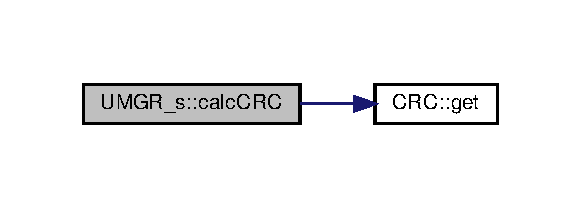
\includegraphics[width=279pt]{structUMGR__s_ae71a2770c3e37f1d859374359f99aae6_cgraph}
\end{center}
\end{figure}
\mbox{\Hypertarget{structUMGR__s_af85ccf0554e33a7f7163c0d26ca791eb}\label{structUMGR__s_af85ccf0554e33a7f7163c0d26ca791eb}} 
\index{U\+M\+G\+R\+\_\+s@{U\+M\+G\+R\+\_\+s}!serialize@{serialize}}
\index{serialize@{serialize}!U\+M\+G\+R\+\_\+s@{U\+M\+G\+R\+\_\+s}}
\subsubsection{\texorpdfstring{serialize()}{serialize()}}
{\footnotesize\ttfamily template$<$typename Archive $>$ \\
void U\+M\+G\+R\+\_\+s\+::serialize (\begin{DoxyParamCaption}\item[{Archive \&}]{ar,  }\item[{const unsigned int}]{version }\end{DoxyParamCaption})\hspace{0.3cm}{\ttfamily [inline]}}



function for serializing the struct 



\subsection{Member Data Documentation}
\mbox{\Hypertarget{structUMGR__s_a3a98cb14c2b8c9545aa47871865076e6}\label{structUMGR__s_a3a98cb14c2b8c9545aa47871865076e6}} 
\index{U\+M\+G\+R\+\_\+s@{U\+M\+G\+R\+\_\+s}!checksum@{checksum}}
\index{checksum@{checksum}!U\+M\+G\+R\+\_\+s@{U\+M\+G\+R\+\_\+s}}
\subsubsection{\texorpdfstring{checksum}{checksum}}
{\footnotesize\ttfamily int U\+M\+G\+R\+\_\+s\+::checksum}

\mbox{\Hypertarget{structUMGR__s_a80540aaa70f1333ba3c558f6af7a39a1}\label{structUMGR__s_a80540aaa70f1333ba3c558f6af7a39a1}} 
\index{U\+M\+G\+R\+\_\+s@{U\+M\+G\+R\+\_\+s}!description@{description}}
\index{description@{description}!U\+M\+G\+R\+\_\+s@{U\+M\+G\+R\+\_\+s}}
\subsubsection{\texorpdfstring{description}{description}}
{\footnotesize\ttfamily string U\+M\+G\+R\+\_\+s\+::description}

\mbox{\Hypertarget{structUMGR__s_a0a329d092b37dd9061136642d6bebd15}\label{structUMGR__s_a0a329d092b37dd9061136642d6bebd15}} 
\index{U\+M\+G\+R\+\_\+s@{U\+M\+G\+R\+\_\+s}!dlt\+\_\+id@{dlt\+\_\+id}}
\index{dlt\+\_\+id@{dlt\+\_\+id}!U\+M\+G\+R\+\_\+s@{U\+M\+G\+R\+\_\+s}}
\subsubsection{\texorpdfstring{dlt\+\_\+id}{dlt\_id}}
{\footnotesize\ttfamily string U\+M\+G\+R\+\_\+s\+::dlt\+\_\+id}

\mbox{\Hypertarget{structUMGR__s_a9024c1140605de70cf368de635024702}\label{structUMGR__s_a9024c1140605de70cf368de635024702}} 
\index{U\+M\+G\+R\+\_\+s@{U\+M\+G\+R\+\_\+s}!ipc\+\_\+port@{ipc\+\_\+port}}
\index{ipc\+\_\+port@{ipc\+\_\+port}!U\+M\+G\+R\+\_\+s@{U\+M\+G\+R\+\_\+s}}
\subsubsection{\texorpdfstring{ipc\+\_\+port}{ipc\_port}}
{\footnotesize\ttfamily unsigned int U\+M\+G\+R\+\_\+s\+::ipc\+\_\+port}

\mbox{\Hypertarget{structUMGR__s_ae8d842a1050f74d35c2785f9d72f7197}\label{structUMGR__s_ae8d842a1050f74d35c2785f9d72f7197}} 
\index{U\+M\+G\+R\+\_\+s@{U\+M\+G\+R\+\_\+s}!log\+\_\+dir\+\_\+path@{log\+\_\+dir\+\_\+path}}
\index{log\+\_\+dir\+\_\+path@{log\+\_\+dir\+\_\+path}!U\+M\+G\+R\+\_\+s@{U\+M\+G\+R\+\_\+s}}
\subsubsection{\texorpdfstring{log\+\_\+dir\+\_\+path}{log\_dir\_path}}
{\footnotesize\ttfamily string U\+M\+G\+R\+\_\+s\+::log\+\_\+dir\+\_\+path}

\mbox{\Hypertarget{structUMGR__s_a59eaa08e65bbab14ab1deb4969a261c3}\label{structUMGR__s_a59eaa08e65bbab14ab1deb4969a261c3}} 
\index{U\+M\+G\+R\+\_\+s@{U\+M\+G\+R\+\_\+s}!log\+\_\+level@{log\+\_\+level}}
\index{log\+\_\+level@{log\+\_\+level}!U\+M\+G\+R\+\_\+s@{U\+M\+G\+R\+\_\+s}}
\subsubsection{\texorpdfstring{log\+\_\+level}{log\_level}}
{\footnotesize\ttfamily string U\+M\+G\+R\+\_\+s\+::log\+\_\+level}

\mbox{\Hypertarget{structUMGR__s_ab9ebb2767a511f0e791ae1f07b2a03e2}\label{structUMGR__s_ab9ebb2767a511f0e791ae1f07b2a03e2}} 
\index{U\+M\+G\+R\+\_\+s@{U\+M\+G\+R\+\_\+s}!log\+\_\+mode@{log\+\_\+mode}}
\index{log\+\_\+mode@{log\+\_\+mode}!U\+M\+G\+R\+\_\+s@{U\+M\+G\+R\+\_\+s}}
\subsubsection{\texorpdfstring{log\+\_\+mode}{log\_mode}}
{\footnotesize\ttfamily string U\+M\+G\+R\+\_\+s\+::log\+\_\+mode}

\mbox{\Hypertarget{structUMGR__s_aa3ce6d48e8db2d85e084d079548b8338}\label{structUMGR__s_aa3ce6d48e8db2d85e084d079548b8338}} 
\index{U\+M\+G\+R\+\_\+s@{U\+M\+G\+R\+\_\+s}!msg\+\_\+buf\+\_\+size@{msg\+\_\+buf\+\_\+size}}
\index{msg\+\_\+buf\+\_\+size@{msg\+\_\+buf\+\_\+size}!U\+M\+G\+R\+\_\+s@{U\+M\+G\+R\+\_\+s}}
\subsubsection{\texorpdfstring{msg\+\_\+buf\+\_\+size}{msg\_buf\_size}}
{\footnotesize\ttfamily unsigned int U\+M\+G\+R\+\_\+s\+::msg\+\_\+buf\+\_\+size}

\mbox{\Hypertarget{structUMGR__s_a3d36ca5f936e211da7645b00894c68dd}\label{structUMGR__s_a3d36ca5f936e211da7645b00894c68dd}} 
\index{U\+M\+G\+R\+\_\+s@{U\+M\+G\+R\+\_\+s}!name@{name}}
\index{name@{name}!U\+M\+G\+R\+\_\+s@{U\+M\+G\+R\+\_\+s}}
\subsubsection{\texorpdfstring{name}{name}}
{\footnotesize\ttfamily string U\+M\+G\+R\+\_\+s\+::name}

\mbox{\Hypertarget{structUMGR__s_af846433f5bfd716a224c3cf7ac208fdb}\label{structUMGR__s_af846433f5bfd716a224c3cf7ac208fdb}} 
\index{U\+M\+G\+R\+\_\+s@{U\+M\+G\+R\+\_\+s}!reconnection\+\_\+retry\+\_\+offset@{reconnection\+\_\+retry\+\_\+offset}}
\index{reconnection\+\_\+retry\+\_\+offset@{reconnection\+\_\+retry\+\_\+offset}!U\+M\+G\+R\+\_\+s@{U\+M\+G\+R\+\_\+s}}
\subsubsection{\texorpdfstring{reconnection\+\_\+retry\+\_\+offset}{reconnection\_retry\_offset}}
{\footnotesize\ttfamily unsigned int U\+M\+G\+R\+\_\+s\+::reconnection\+\_\+retry\+\_\+offset}



The documentation for this struct was generated from the following file\+:\begin{DoxyCompactItemize}
\item 
/home/visxim/\+C\+Lion\+Projects/\+Adaptive\+Dummy\+Process/includes/\hyperlink{data__storage_8h}{data\+\_\+storage.\+h}\end{DoxyCompactItemize}

\chapter{File Documentation}
\hypertarget{checksum__manager_8cpp}{}\section{/home/visxim/\+C\+Lion\+Projects/\+Adaptive\+Dummy\+Process/checksum\+\_\+manager.cpp File Reference}
\label{checksum__manager_8cpp}\index{/home/visxim/\+C\+Lion\+Projects/\+Adaptive\+Dummy\+Process/checksum\+\_\+manager.\+cpp@{/home/visxim/\+C\+Lion\+Projects/\+Adaptive\+Dummy\+Process/checksum\+\_\+manager.\+cpp}}


Checksum\+\_\+manager for checking the integrity of the data.  


{\ttfamily \#include \char`\"{}checksum\+\_\+manager.\+h\char`\"{}}\newline
Include dependency graph for checksum\+\_\+manager.\+cpp\+:
\nopagebreak
\begin{figure}[H]
\begin{center}
\leavevmode
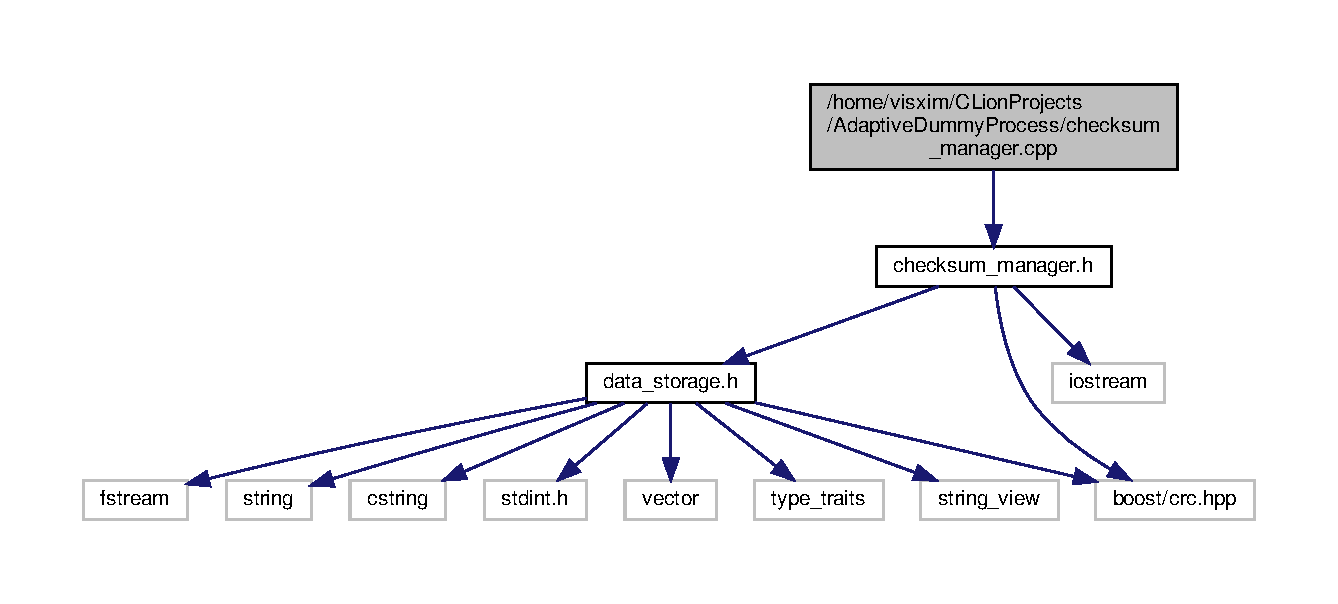
\includegraphics[width=350pt]{checksum__manager_8cpp__incl}
\end{center}
\end{figure}


\subsection{Detailed Description}
Checksum\+\_\+manager for checking the integrity of the data. 

The Checksum\+\_\+manager creates and checks if the data is valid 
\hypertarget{deserializer_8cpp}{}\section{/home/visxim/\+C\+Lion\+Projects/\+Adaptive\+Dummy\+Process/deserializer.cpp File Reference}
\label{deserializer_8cpp}\index{/home/visxim/\+C\+Lion\+Projects/\+Adaptive\+Dummy\+Process/deserializer.\+cpp@{/home/visxim/\+C\+Lion\+Projects/\+Adaptive\+Dummy\+Process/deserializer.\+cpp}}


Deserializer for deserializing the parsed configuration data.  


{\ttfamily \#include \char`\"{}deserializer.\+h\char`\"{}}\newline
Include dependency graph for deserializer.\+cpp\+:
\nopagebreak
\begin{figure}[H]
\begin{center}
\leavevmode
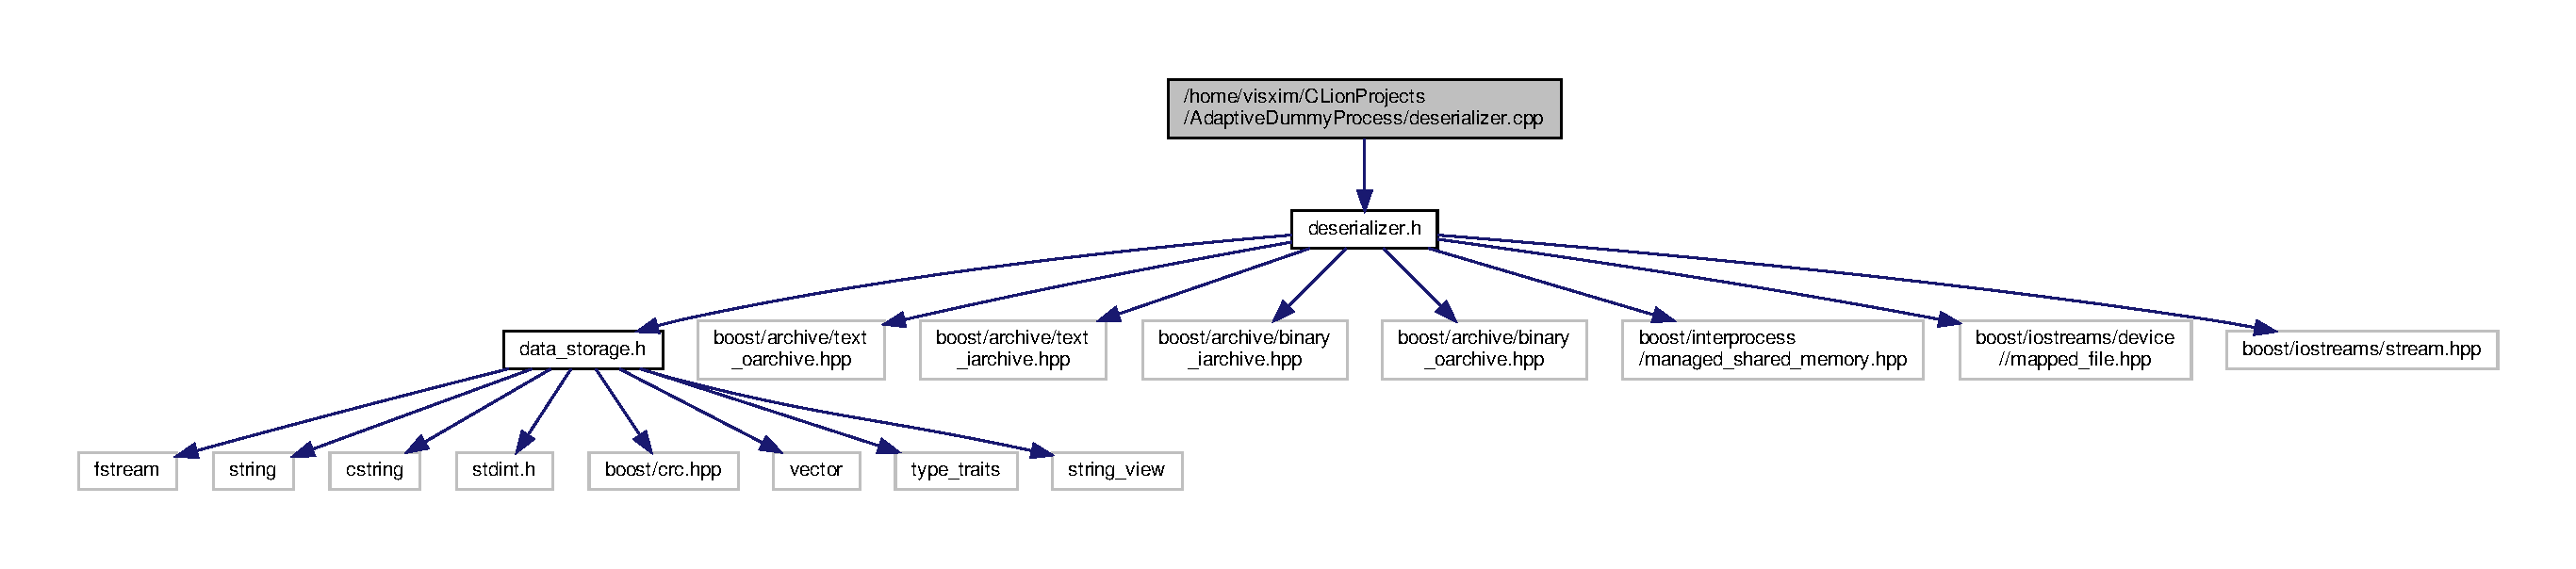
\includegraphics[width=350pt]{deserializer_8cpp__incl}
\end{center}
\end{figure}


\subsection{Detailed Description}
Deserializer for deserializing the parsed configuration data. 

Deserializer for deserializing data from both shared memory and files 
\hypertarget{checksum__manager_8h}{}\section{/home/visxim/\+C\+Lion\+Projects/\+Adaptive\+Dummy\+Process/includes/checksum\+\_\+manager.h File Reference}
\label{checksum__manager_8h}\index{/home/visxim/\+C\+Lion\+Projects/\+Adaptive\+Dummy\+Process/includes/checksum\+\_\+manager.\+h@{/home/visxim/\+C\+Lion\+Projects/\+Adaptive\+Dummy\+Process/includes/checksum\+\_\+manager.\+h}}


Header of \hyperlink{classchecksum__manager}{checksum\+\_\+manager} for checking the integrity of the data.  


{\ttfamily \#include \char`\"{}data\+\_\+storage.\+h\char`\"{}}\newline
{\ttfamily \#include \char`\"{}boost/crc.\+hpp\char`\"{}}\newline
{\ttfamily \#include $<$iostream$>$}\newline
Include dependency graph for checksum\+\_\+manager.\+h\+:
\nopagebreak
\begin{figure}[H]
\begin{center}
\leavevmode
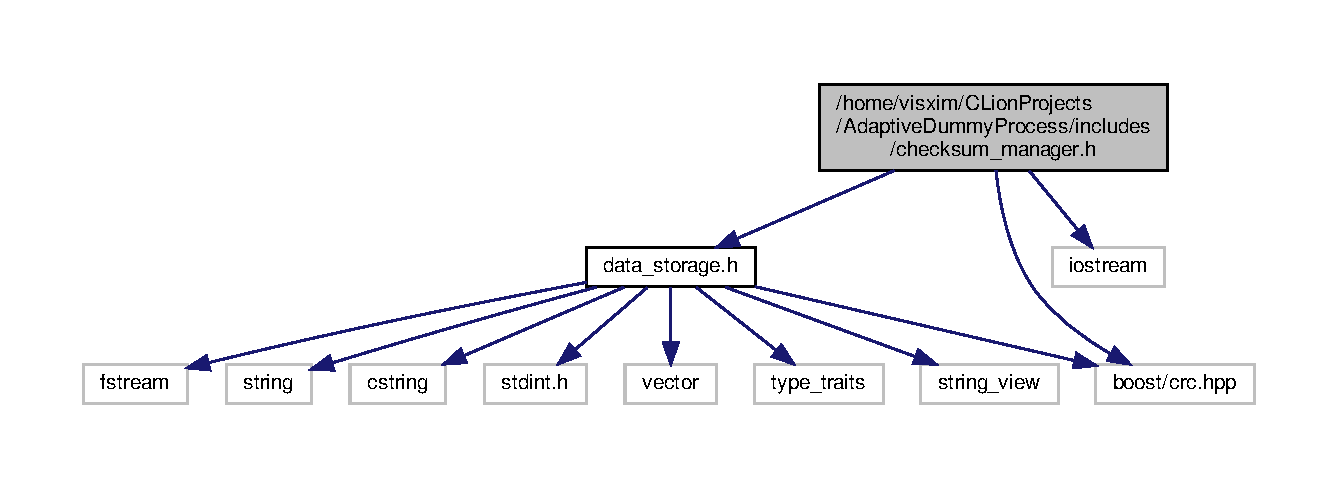
\includegraphics[width=350pt]{checksum__manager_8h__incl}
\end{center}
\end{figure}
This graph shows which files directly or indirectly include this file\+:
\nopagebreak
\begin{figure}[H]
\begin{center}
\leavevmode
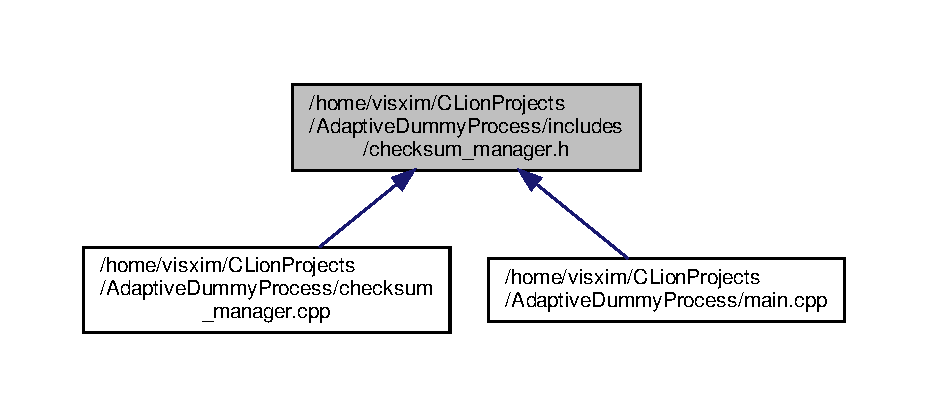
\includegraphics[width=350pt]{checksum__manager_8h__dep__incl}
\end{center}
\end{figure}
\subsection*{Classes}
\begin{DoxyCompactItemize}
\item 
class \hyperlink{classchecksum__manager}{checksum\+\_\+manager}
\begin{DoxyCompactList}\small\item\em Class of checksum manager for \hyperlink{structCRC}{C\+RC} managment. \end{DoxyCompactList}\end{DoxyCompactItemize}


\subsection{Detailed Description}
Header of \hyperlink{classchecksum__manager}{checksum\+\_\+manager} for checking the integrity of the data. 

The Checksum\+\_\+manager creates and checks if the data is valid 
\hypertarget{data__storage_8h}{}\section{/home/visxim/\+C\+Lion\+Projects/\+Adaptive\+Dummy\+Process/includes/data\+\_\+storage.h File Reference}
\label{data__storage_8h}\index{/home/visxim/\+C\+Lion\+Projects/\+Adaptive\+Dummy\+Process/includes/data\+\_\+storage.\+h@{/home/visxim/\+C\+Lion\+Projects/\+Adaptive\+Dummy\+Process/includes/data\+\_\+storage.\+h}}


Header of \hyperlink{classchecksum__manager}{checksum\+\_\+manager} for checking the integrity of the data.  


{\ttfamily \#include $<$fstream$>$}\newline
{\ttfamily \#include $<$string$>$}\newline
{\ttfamily \#include $<$cstring$>$}\newline
{\ttfamily \#include $<$stdint.\+h$>$}\newline
{\ttfamily \#include \char`\"{}boost/crc.\+hpp\char`\"{}}\newline
{\ttfamily \#include $<$vector$>$}\newline
{\ttfamily \#include $<$type\+\_\+traits$>$}\newline
{\ttfamily \#include $<$string\+\_\+view$>$}\newline
Include dependency graph for data\+\_\+storage.\+h\+:
\nopagebreak
\begin{figure}[H]
\begin{center}
\leavevmode
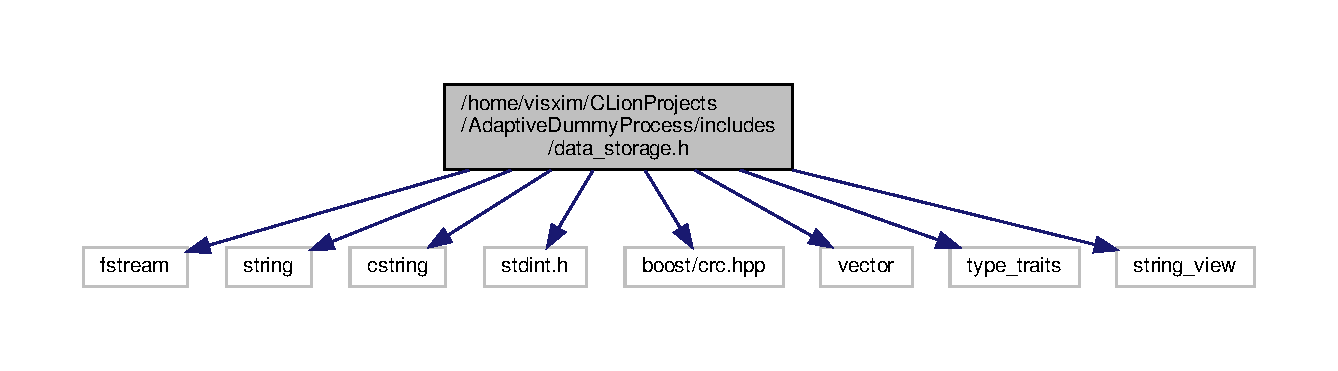
\includegraphics[width=350pt]{data__storage_8h__incl}
\end{center}
\end{figure}
This graph shows which files directly or indirectly include this file\+:
\nopagebreak
\begin{figure}[H]
\begin{center}
\leavevmode
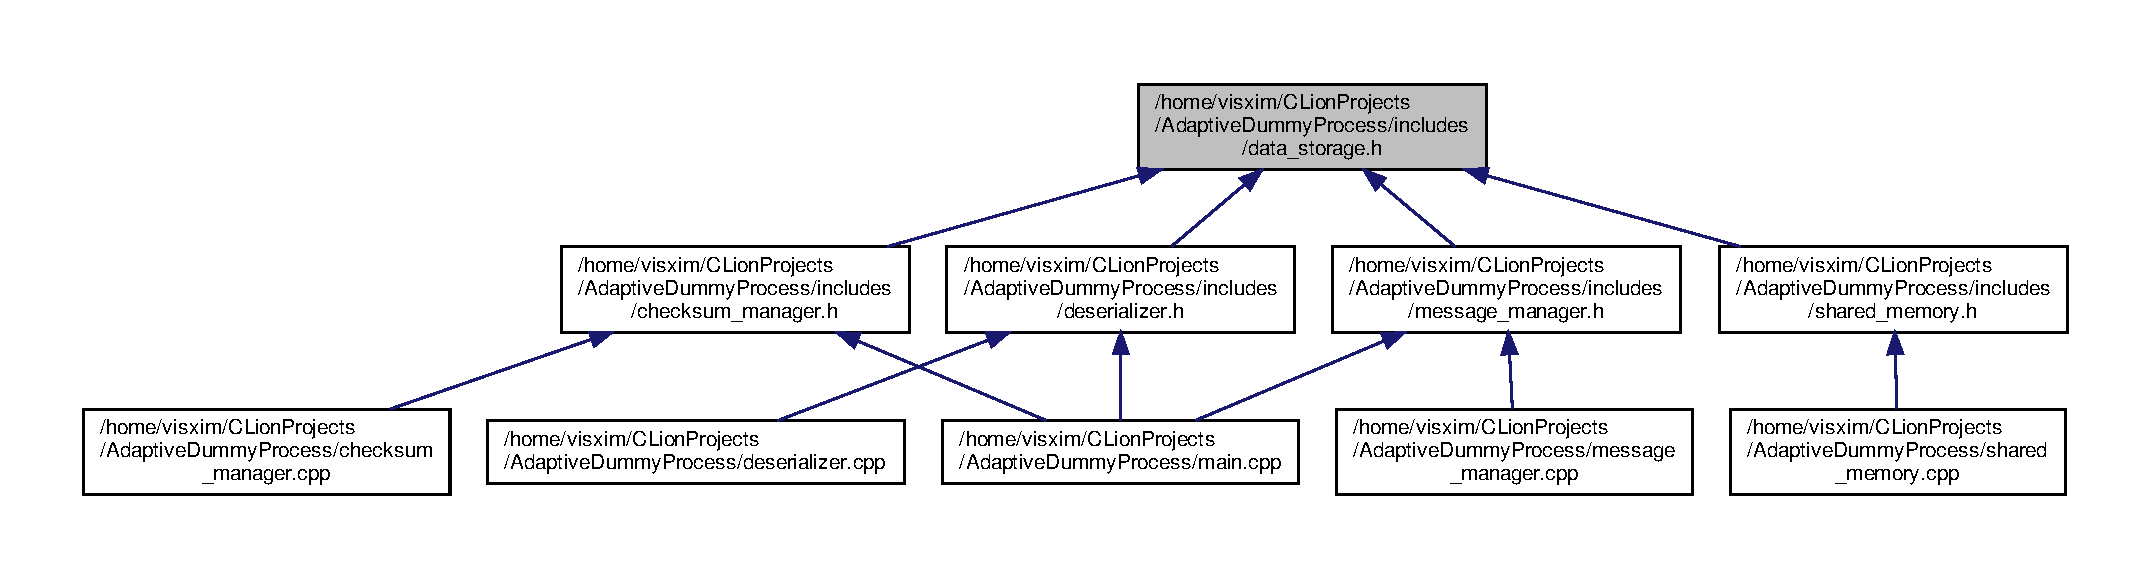
\includegraphics[width=350pt]{data__storage_8h__dep__incl}
\end{center}
\end{figure}
\subsection*{Classes}
\begin{DoxyCompactItemize}
\item 
struct \hyperlink{structCRC}{C\+RC}
\item 
struct \hyperlink{structUMGR__s}{U\+M\+G\+R\+\_\+s}
\begin{DoxyCompactList}\small\item\em Struct which is specified to hold the values of the Update\+Manager U\+M\+GR. \end{DoxyCompactList}\item 
struct \hyperlink{structEXMPLE__s}{E\+X\+M\+P\+L\+E\+\_\+s}
\end{DoxyCompactItemize}


\subsection{Detailed Description}
Header of \hyperlink{classchecksum__manager}{checksum\+\_\+manager} for checking the integrity of the data. 

The Checksum\+\_\+manager creates and checks if the data is valid 
\hypertarget{deserializer_8h}{}\section{/home/visxim/\+C\+Lion\+Projects/\+Adaptive\+Dummy\+Process/includes/deserializer.h File Reference}
\label{deserializer_8h}\index{/home/visxim/\+C\+Lion\+Projects/\+Adaptive\+Dummy\+Process/includes/deserializer.\+h@{/home/visxim/\+C\+Lion\+Projects/\+Adaptive\+Dummy\+Process/includes/deserializer.\+h}}


Header of deserializer for deserializing the parsed configuration data.  


{\ttfamily \#include \char`\"{}data\+\_\+storage.\+h\char`\"{}}\newline
{\ttfamily \#include $<$boost/archive/text\+\_\+oarchive.\+hpp$>$}\newline
{\ttfamily \#include $<$boost/archive/text\+\_\+iarchive.\+hpp$>$}\newline
{\ttfamily \#include $<$boost/archive/binary\+\_\+iarchive.\+hpp$>$}\newline
{\ttfamily \#include $<$boost/archive/binary\+\_\+oarchive.\+hpp$>$}\newline
{\ttfamily \#include $<$boost/interprocess/managed\+\_\+shared\+\_\+memory.\+hpp$>$}\newline
{\ttfamily \#include $<$boost/iostreams/device//mapped\+\_\+file.\+hpp$>$}\newline
{\ttfamily \#include $<$boost/iostreams/stream.\+hpp$>$}\newline
Include dependency graph for deserializer.\+h\+:
\nopagebreak
\begin{figure}[H]
\begin{center}
\leavevmode
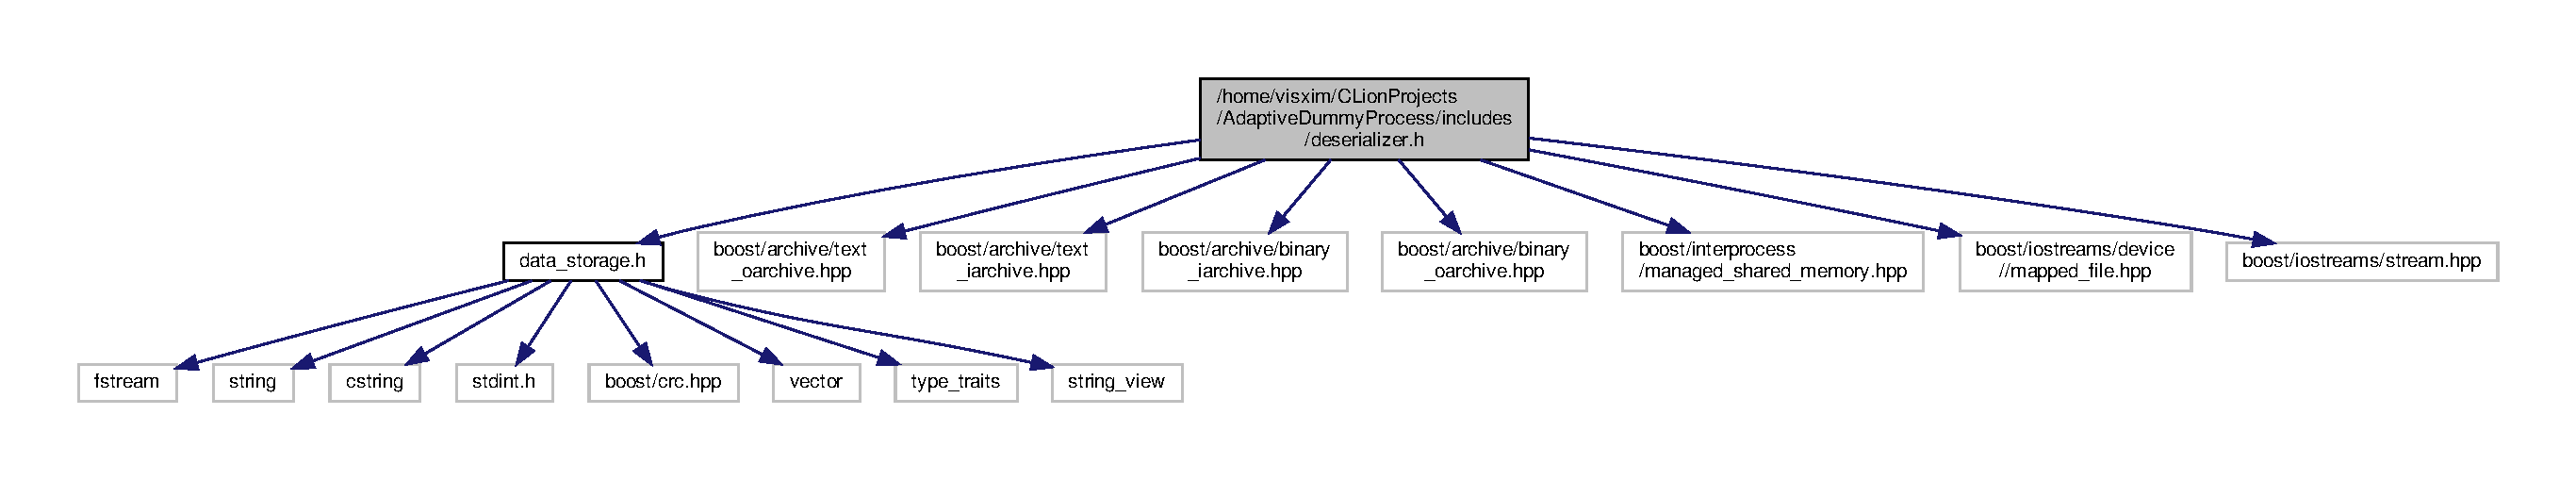
\includegraphics[width=350pt]{deserializer_8h__incl}
\end{center}
\end{figure}
This graph shows which files directly or indirectly include this file\+:
\nopagebreak
\begin{figure}[H]
\begin{center}
\leavevmode
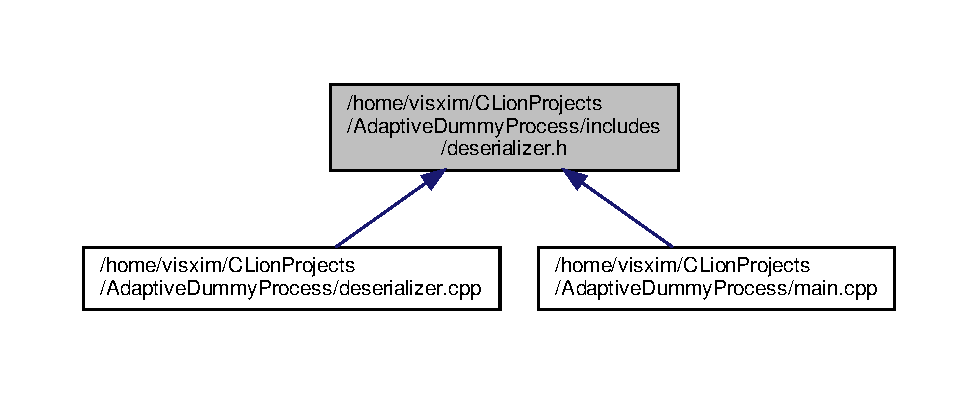
\includegraphics[width=350pt]{deserializer_8h__dep__incl}
\end{center}
\end{figure}
\subsection*{Classes}
\begin{DoxyCompactItemize}
\item 
class \hyperlink{classdeserializer}{deserializer}
\begin{DoxyCompactList}\small\item\em Class of deserializer which handles deserialization of data from files and shared memory. \end{DoxyCompactList}\end{DoxyCompactItemize}


\subsection{Detailed Description}
Header of deserializer for deserializing the parsed configuration data. 

Deserializer for deserializing data from both shared memory and files 
\hypertarget{message__manager_8h}{}\section{/home/visxim/\+C\+Lion\+Projects/\+Adaptive\+Dummy\+Process/includes/message\+\_\+manager.h File Reference}
\label{message__manager_8h}\index{/home/visxim/\+C\+Lion\+Projects/\+Adaptive\+Dummy\+Process/includes/message\+\_\+manager.\+h@{/home/visxim/\+C\+Lion\+Projects/\+Adaptive\+Dummy\+Process/includes/message\+\_\+manager.\+h}}


Header of \hyperlink{classmessage__manager}{message\+\_\+manager} for managing the synchronization between processes.  


{\ttfamily \#include $<$iostream$>$}\newline
{\ttfamily \#include \char`\"{}boost/interprocess/ipc/message\+\_\+queue.\+hpp\char`\"{}}\newline
{\ttfamily \#include \char`\"{}boost/scoped\+\_\+ptr.\+hpp\char`\"{}}\newline
{\ttfamily \#include \char`\"{}data\+\_\+storage.\+h\char`\"{}}\newline
Include dependency graph for message\+\_\+manager.\+h\+:
\nopagebreak
\begin{figure}[H]
\begin{center}
\leavevmode
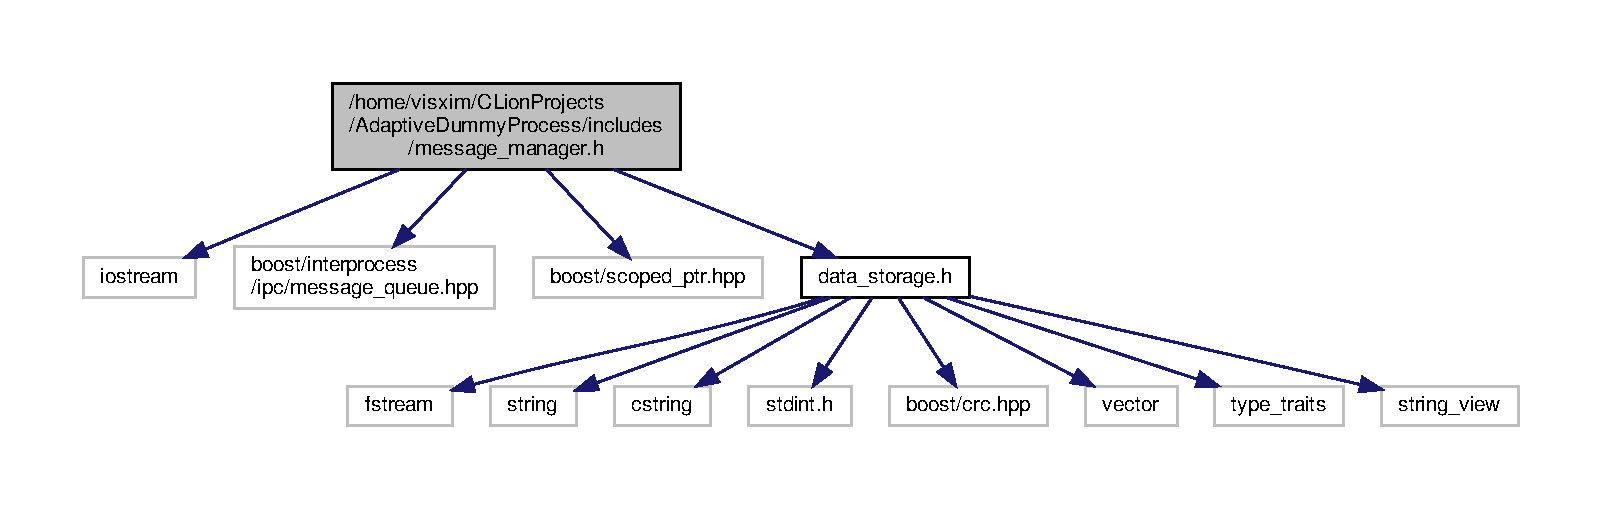
\includegraphics[width=350pt]{message__manager_8h__incl}
\end{center}
\end{figure}
This graph shows which files directly or indirectly include this file\+:
\nopagebreak
\begin{figure}[H]
\begin{center}
\leavevmode
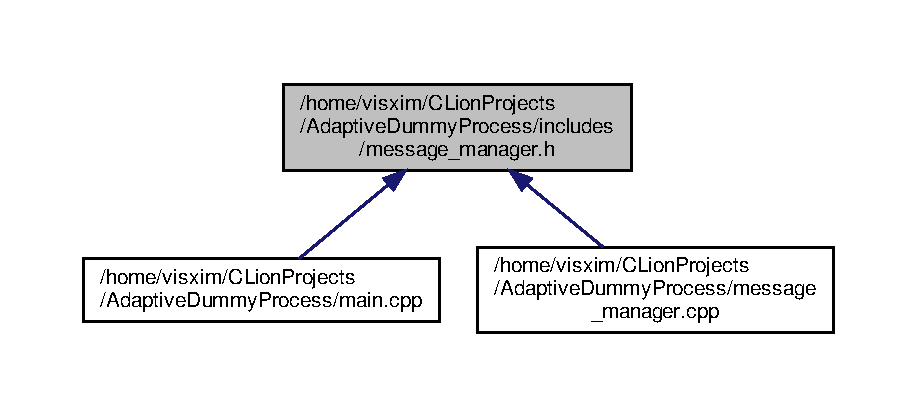
\includegraphics[width=350pt]{message__manager_8h__dep__incl}
\end{center}
\end{figure}
\subsection*{Classes}
\begin{DoxyCompactItemize}
\item 
class \hyperlink{classmessage__manager}{message\+\_\+manager}
\begin{DoxyCompactList}\small\item\em Class of message manager which handles the synchronization between processes. \end{DoxyCompactList}\end{DoxyCompactItemize}


\subsection{Detailed Description}
Header of \hyperlink{classmessage__manager}{message\+\_\+manager} for managing the synchronization between processes. 

The \hyperlink{classmessage__manager}{message\+\_\+manager} managed all synchronization between processes via message queue 
\hypertarget{shared__memory_8h}{}\section{/home/visxim/\+C\+Lion\+Projects/\+Adaptive\+Dummy\+Process/includes/shared\+\_\+memory.h File Reference}
\label{shared__memory_8h}\index{/home/visxim/\+C\+Lion\+Projects/\+Adaptive\+Dummy\+Process/includes/shared\+\_\+memory.\+h@{/home/visxim/\+C\+Lion\+Projects/\+Adaptive\+Dummy\+Process/includes/shared\+\_\+memory.\+h}}
{\ttfamily \#include \char`\"{}data\+\_\+storage.\+h\char`\"{}}\newline
{\ttfamily \#include $<$boost/interprocess/managed\+\_\+shared\+\_\+memory.\+hpp$>$}\newline
Include dependency graph for shared\+\_\+memory.\+h\+:
\nopagebreak
\begin{figure}[H]
\begin{center}
\leavevmode
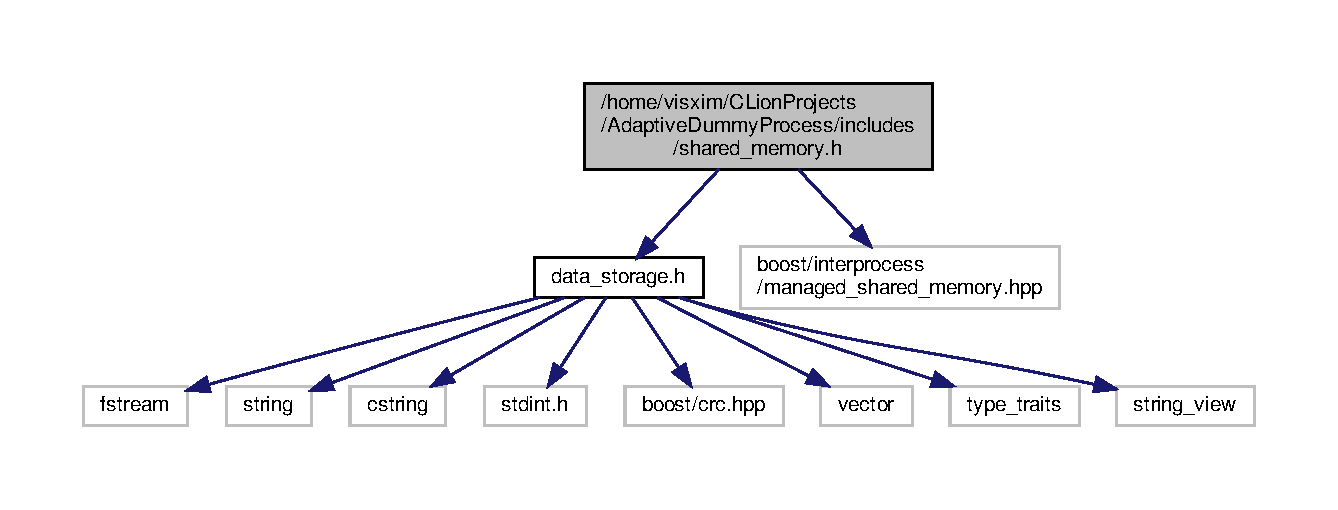
\includegraphics[width=350pt]{shared__memory_8h__incl}
\end{center}
\end{figure}
This graph shows which files directly or indirectly include this file\+:
\nopagebreak
\begin{figure}[H]
\begin{center}
\leavevmode
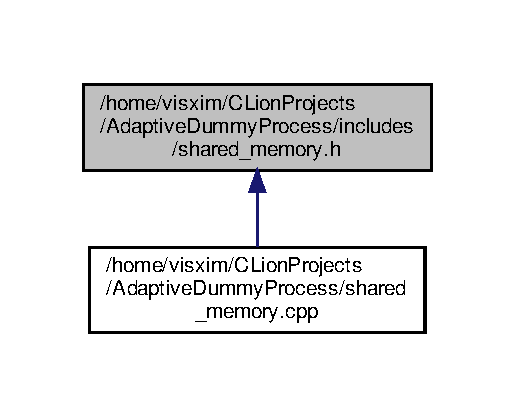
\includegraphics[width=247pt]{shared__memory_8h__dep__incl}
\end{center}
\end{figure}
\subsection*{Classes}
\begin{DoxyCompactItemize}
\item 
class \hyperlink{classshared__memory}{shared\+\_\+memory}
\end{DoxyCompactItemize}

\hypertarget{time-tp_8h}{}\section{/home/visxim/\+C\+Lion\+Projects/\+Adaptive\+Dummy\+Process/includes/time-\/tp.h File Reference}
\label{time-tp_8h}\index{/home/visxim/\+C\+Lion\+Projects/\+Adaptive\+Dummy\+Process/includes/time-\/tp.\+h@{/home/visxim/\+C\+Lion\+Projects/\+Adaptive\+Dummy\+Process/includes/time-\/tp.\+h}}
{\ttfamily \#include $<$lttng/tracepoint.\+h$>$}\newline
{\ttfamily \#include $<$lttng/tracepoint-\/event.\+h$>$}\newline
Include dependency graph for time-\/tp.h\+:
\nopagebreak
\begin{figure}[H]
\begin{center}
\leavevmode
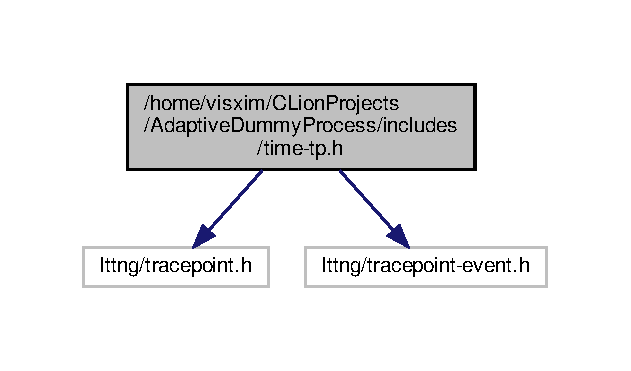
\includegraphics[width=303pt]{time-tp_8h__incl}
\end{center}
\end{figure}
This graph shows which files directly or indirectly include this file\+:
\nopagebreak
\begin{figure}[H]
\begin{center}
\leavevmode
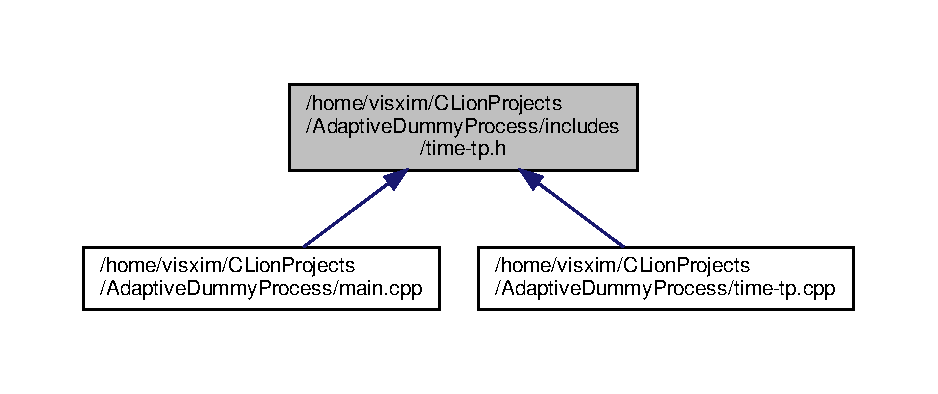
\includegraphics[width=350pt]{time-tp_8h__dep__incl}
\end{center}
\end{figure}
\subsection*{Macros}
\begin{DoxyCompactItemize}
\item 
\#define \hyperlink{time-tp_8h_a6751837690af3a0ad19fb209a69dd16e}{T\+R\+A\+C\+E\+P\+O\+I\+N\+T\+\_\+\+P\+R\+O\+V\+I\+D\+ER}~tp\+\_\+provider
\item 
\#define \hyperlink{time-tp_8h_a090261faa16d05fb6993d61861ba8ff9}{T\+R\+A\+C\+E\+P\+O\+I\+N\+T\+\_\+\+I\+N\+C\+L\+U\+DE}~\char`\"{}./time-\/tp.\+h\char`\"{}
\item 
\#define \hyperlink{time-tp_8h_ad91ef7d5cc408393bcfaf376512d4ce7}{\+\_\+time\+\_\+\+T\+P\+\_\+H}
\item 
\#define \hyperlink{time-tp_8h_a36d219a400a7a885e95c8e51318b4180}{T\+R\+A\+C\+E\+O\+L\+D\+F\+I\+LE}
\begin{DoxyCompactList}\small\item\em Defines if tracing is enabled. \end{DoxyCompactList}\end{DoxyCompactItemize}
\subsection*{Functions}
\begin{DoxyCompactItemize}
\item 
\hyperlink{time-tp_8h_a2b7f574c00f7fe1cbd4b66ccca5e2fab}{T\+R\+A\+C\+E\+P\+O\+I\+N\+T\+\_\+\+E\+V\+E\+NT} (tp\+\_\+provider, time\+\_\+tracepoint\+\_\+dummy\+\_\+old, \hyperlink{time-tp_8h_a94a7a81b68dcdbeece169da86213a640}{T\+P\+\_\+\+A\+R\+GS}(int, probe\+\_\+nr), T\+P\+\_\+\+F\+I\+E\+L\+DS(ctf\+\_\+integer(int, probe\+Number, probe\+\_\+nr))) T\+R\+A\+C\+E\+P\+O\+I\+N\+T\+\_\+\+E\+V\+E\+NT(tp\+\_\+provider
\item 
\hyperlink{time-tp_8h_a94a7a81b68dcdbeece169da86213a640}{T\+P\+\_\+\+A\+R\+GS} (int, probe\+\_\+nr)
\end{DoxyCompactItemize}
\subsection*{Variables}
\begin{DoxyCompactItemize}
\item 
\hyperlink{time-tp_8h_a5bbda58654652cd1266ef94415814b2d}{time\+\_\+tracepoint\+\_\+dummy\+\_\+new}
\end{DoxyCompactItemize}


\subsection{Macro Definition Documentation}
\mbox{\Hypertarget{time-tp_8h_ad91ef7d5cc408393bcfaf376512d4ce7}\label{time-tp_8h_ad91ef7d5cc408393bcfaf376512d4ce7}} 
\index{time-\/tp.\+h@{time-\/tp.\+h}!\+\_\+time\+\_\+\+T\+P\+\_\+H@{\+\_\+time\+\_\+\+T\+P\+\_\+H}}
\index{\+\_\+time\+\_\+\+T\+P\+\_\+H@{\+\_\+time\+\_\+\+T\+P\+\_\+H}!time-\/tp.\+h@{time-\/tp.\+h}}
\subsubsection{\texorpdfstring{\+\_\+time\+\_\+\+T\+P\+\_\+H}{\_time\_TP\_H}}
{\footnotesize\ttfamily \#define \+\_\+time\+\_\+\+T\+P\+\_\+H}

\mbox{\Hypertarget{time-tp_8h_a36d219a400a7a885e95c8e51318b4180}\label{time-tp_8h_a36d219a400a7a885e95c8e51318b4180}} 
\index{time-\/tp.\+h@{time-\/tp.\+h}!T\+R\+A\+C\+E\+O\+L\+D\+F\+I\+LE@{T\+R\+A\+C\+E\+O\+L\+D\+F\+I\+LE}}
\index{T\+R\+A\+C\+E\+O\+L\+D\+F\+I\+LE@{T\+R\+A\+C\+E\+O\+L\+D\+F\+I\+LE}!time-\/tp.\+h@{time-\/tp.\+h}}
\subsubsection{\texorpdfstring{T\+R\+A\+C\+E\+O\+L\+D\+F\+I\+LE}{TRACEOLDFILE}}
{\footnotesize\ttfamily \#define T\+R\+A\+C\+E\+O\+L\+D\+F\+I\+LE}



Defines if tracing is enabled. 

\mbox{\Hypertarget{time-tp_8h_a090261faa16d05fb6993d61861ba8ff9}\label{time-tp_8h_a090261faa16d05fb6993d61861ba8ff9}} 
\index{time-\/tp.\+h@{time-\/tp.\+h}!T\+R\+A\+C\+E\+P\+O\+I\+N\+T\+\_\+\+I\+N\+C\+L\+U\+DE@{T\+R\+A\+C\+E\+P\+O\+I\+N\+T\+\_\+\+I\+N\+C\+L\+U\+DE}}
\index{T\+R\+A\+C\+E\+P\+O\+I\+N\+T\+\_\+\+I\+N\+C\+L\+U\+DE@{T\+R\+A\+C\+E\+P\+O\+I\+N\+T\+\_\+\+I\+N\+C\+L\+U\+DE}!time-\/tp.\+h@{time-\/tp.\+h}}
\subsubsection{\texorpdfstring{T\+R\+A\+C\+E\+P\+O\+I\+N\+T\+\_\+\+I\+N\+C\+L\+U\+DE}{TRACEPOINT\_INCLUDE}}
{\footnotesize\ttfamily \#define T\+R\+A\+C\+E\+P\+O\+I\+N\+T\+\_\+\+I\+N\+C\+L\+U\+DE~\char`\"{}./time-\/tp.\+h\char`\"{}}

\mbox{\Hypertarget{time-tp_8h_a6751837690af3a0ad19fb209a69dd16e}\label{time-tp_8h_a6751837690af3a0ad19fb209a69dd16e}} 
\index{time-\/tp.\+h@{time-\/tp.\+h}!T\+R\+A\+C\+E\+P\+O\+I\+N\+T\+\_\+\+P\+R\+O\+V\+I\+D\+ER@{T\+R\+A\+C\+E\+P\+O\+I\+N\+T\+\_\+\+P\+R\+O\+V\+I\+D\+ER}}
\index{T\+R\+A\+C\+E\+P\+O\+I\+N\+T\+\_\+\+P\+R\+O\+V\+I\+D\+ER@{T\+R\+A\+C\+E\+P\+O\+I\+N\+T\+\_\+\+P\+R\+O\+V\+I\+D\+ER}!time-\/tp.\+h@{time-\/tp.\+h}}
\subsubsection{\texorpdfstring{T\+R\+A\+C\+E\+P\+O\+I\+N\+T\+\_\+\+P\+R\+O\+V\+I\+D\+ER}{TRACEPOINT\_PROVIDER}}
{\footnotesize\ttfamily \#define T\+R\+A\+C\+E\+P\+O\+I\+N\+T\+\_\+\+P\+R\+O\+V\+I\+D\+ER~tp\+\_\+provider}



\subsection{Function Documentation}
\mbox{\Hypertarget{time-tp_8h_a94a7a81b68dcdbeece169da86213a640}\label{time-tp_8h_a94a7a81b68dcdbeece169da86213a640}} 
\index{time-\/tp.\+h@{time-\/tp.\+h}!T\+P\+\_\+\+A\+R\+GS@{T\+P\+\_\+\+A\+R\+GS}}
\index{T\+P\+\_\+\+A\+R\+GS@{T\+P\+\_\+\+A\+R\+GS}!time-\/tp.\+h@{time-\/tp.\+h}}
\subsubsection{\texorpdfstring{T\+P\+\_\+\+A\+R\+G\+S()}{TP\_ARGS()}}
{\footnotesize\ttfamily T\+P\+\_\+\+A\+R\+GS (\begin{DoxyParamCaption}\item[{int}]{,  }\item[{probe\+\_\+nr}]{ }\end{DoxyParamCaption})}

\mbox{\Hypertarget{time-tp_8h_a2b7f574c00f7fe1cbd4b66ccca5e2fab}\label{time-tp_8h_a2b7f574c00f7fe1cbd4b66ccca5e2fab}} 
\index{time-\/tp.\+h@{time-\/tp.\+h}!T\+R\+A\+C\+E\+P\+O\+I\+N\+T\+\_\+\+E\+V\+E\+NT@{T\+R\+A\+C\+E\+P\+O\+I\+N\+T\+\_\+\+E\+V\+E\+NT}}
\index{T\+R\+A\+C\+E\+P\+O\+I\+N\+T\+\_\+\+E\+V\+E\+NT@{T\+R\+A\+C\+E\+P\+O\+I\+N\+T\+\_\+\+E\+V\+E\+NT}!time-\/tp.\+h@{time-\/tp.\+h}}
\subsubsection{\texorpdfstring{T\+R\+A\+C\+E\+P\+O\+I\+N\+T\+\_\+\+E\+V\+E\+N\+T()}{TRACEPOINT\_EVENT()}}
{\footnotesize\ttfamily T\+R\+A\+C\+E\+P\+O\+I\+N\+T\+\_\+\+E\+V\+E\+NT (\begin{DoxyParamCaption}\item[{tp\+\_\+provider}]{,  }\item[{time\+\_\+tracepoint\+\_\+dummy\+\_\+old}]{,  }\item[{\hyperlink{time-tp_8h_a94a7a81b68dcdbeece169da86213a640}{T\+P\+\_\+\+A\+R\+GS}( int, probe\+\_\+nr)}]{,  }\item[{T\+P\+\_\+\+F\+I\+E\+L\+DS( ctf\+\_\+integer(int, probe\+Number, probe\+\_\+nr))}]{ }\end{DoxyParamCaption})}



\subsection{Variable Documentation}
\mbox{\Hypertarget{time-tp_8h_a5bbda58654652cd1266ef94415814b2d}\label{time-tp_8h_a5bbda58654652cd1266ef94415814b2d}} 
\index{time-\/tp.\+h@{time-\/tp.\+h}!time\+\_\+tracepoint\+\_\+dummy\+\_\+new@{time\+\_\+tracepoint\+\_\+dummy\+\_\+new}}
\index{time\+\_\+tracepoint\+\_\+dummy\+\_\+new@{time\+\_\+tracepoint\+\_\+dummy\+\_\+new}!time-\/tp.\+h@{time-\/tp.\+h}}
\subsubsection{\texorpdfstring{time\+\_\+tracepoint\+\_\+dummy\+\_\+new}{time\_tracepoint\_dummy\_new}}
{\footnotesize\ttfamily time\+\_\+tracepoint\+\_\+dummy\+\_\+new}


\hypertarget{main_8cpp}{}\section{/home/visxim/\+C\+Lion\+Projects/\+Adaptive\+Dummy\+Process/main.cpp File Reference}
\label{main_8cpp}\index{/home/visxim/\+C\+Lion\+Projects/\+Adaptive\+Dummy\+Process/main.\+cpp@{/home/visxim/\+C\+Lion\+Projects/\+Adaptive\+Dummy\+Process/main.\+cpp}}


main of the Adaptive\+Dummy\+Process  


{\ttfamily \#include $<$iostream$>$}\newline
{\ttfamily \#include \char`\"{}message\+\_\+manager.\+h\char`\"{}}\newline
{\ttfamily \#include \char`\"{}deserializer.\+h\char`\"{}}\newline
{\ttfamily \#include \char`\"{}checksum\+\_\+manager.\+h\char`\"{}}\newline
{\ttfamily \#include \char`\"{}time-\/tp.\+h\char`\"{}}\newline
Include dependency graph for main.\+cpp\+:
\nopagebreak
\begin{figure}[H]
\begin{center}
\leavevmode
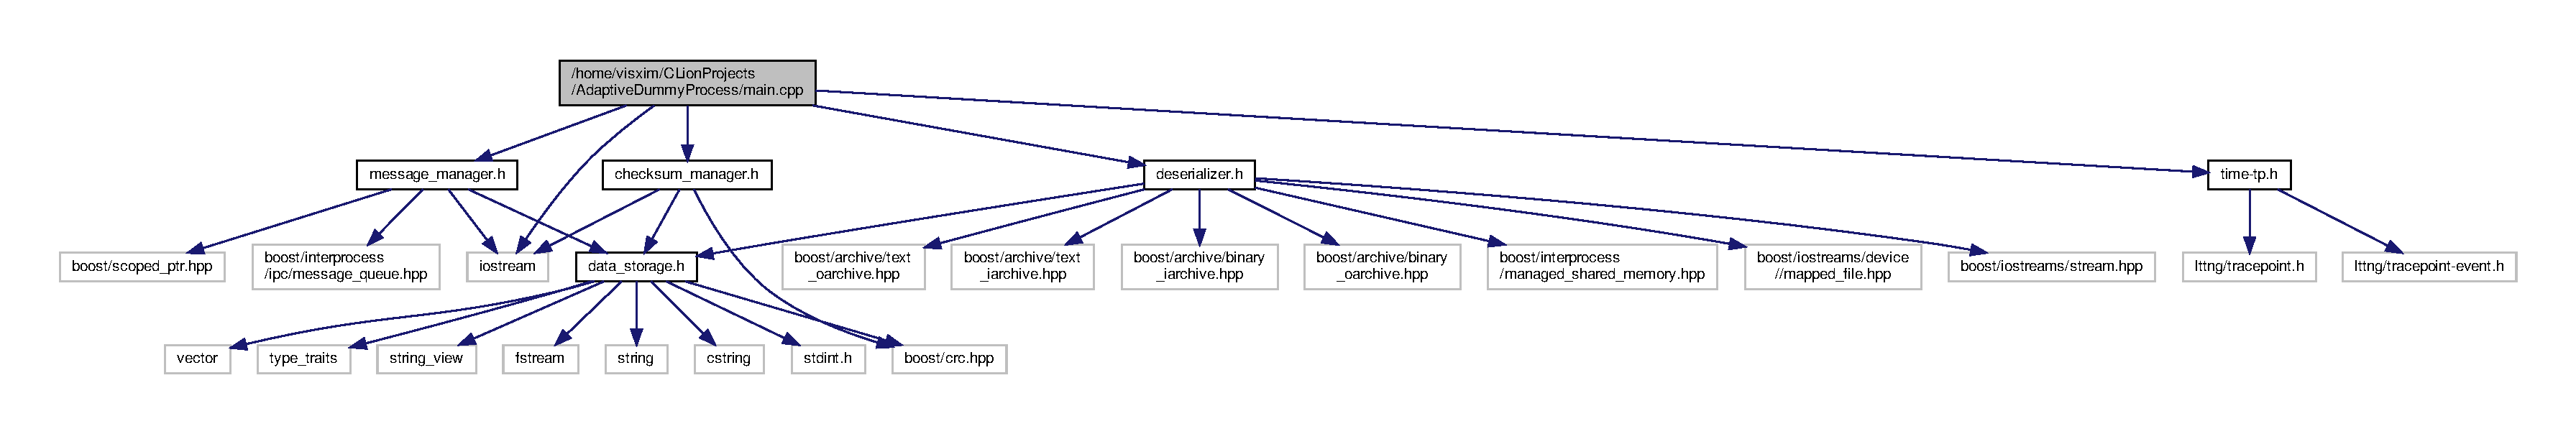
\includegraphics[width=350pt]{main_8cpp__incl}
\end{center}
\end{figure}
\subsection*{Macros}
\begin{DoxyCompactItemize}
\item 
\#define \hyperlink{main_8cpp_a25e7852941475e51c875632ac1985d8a}{P\+R\+I\+O\+R\+I\+TY}~1
\begin{DoxyCompactList}\small\item\em Message\+Queue Priority. \end{DoxyCompactList}\item 
\#define \hyperlink{main_8cpp_afe194f87b759e2541681cfc7bb9a3d72}{E\+X\+M\+P\+LE}
\end{DoxyCompactItemize}
\subsection*{Enumerations}
\begin{DoxyCompactItemize}
\item 
enum \hyperlink{main_8cpp_a1f035773fc136ce529c9c22f3953f7c9}{Sync\+Msg} \{ \newline
\hyperlink{main_8cpp_a1f035773fc136ce529c9c22f3953f7c9a2b8773a31e7caeffc27df2c78df7bd3a}{Process\+Timeout} = 00, 
\hyperlink{main_8cpp_a1f035773fc136ce529c9c22f3953f7c9ac9780f79be0e3d433adeb055d70a4ef6}{Process\+Ready} = 11, 
\hyperlink{main_8cpp_a1f035773fc136ce529c9c22f3953f7c9a3f1f1c2def7164cf1b9b525c6754ec59}{Data\+Rdy\+S\+HM} = 22, 
\hyperlink{main_8cpp_a1f035773fc136ce529c9c22f3953f7c9afc92e28c7aac0d36a3de10fd16c2f6e9}{Data\+Rdy\+File} = 33, 
\newline
\hyperlink{main_8cpp_a1f035773fc136ce529c9c22f3953f7c9a70c465830655f986848e14567e3a0992}{Data\+Receive\+Success} = 44, 
\hyperlink{main_8cpp_a1f035773fc136ce529c9c22f3953f7c9add9875ee9a2249b033cf9a59afba954d}{Data\+Error\+C\+RC} = 55, 
\hyperlink{main_8cpp_a1f035773fc136ce529c9c22f3953f7c9ad970cf97730e7c404d0bf7c460f753df}{Receiving\+Error} = 66, 
\hyperlink{main_8cpp_a1f035773fc136ce529c9c22f3953f7c9aa343c85c32133b3cca6bc019bf6386c4}{Daemon\+Timeout} = 77
 \}\begin{DoxyCompactList}\small\item\em Enum for synchronization via message queue. \end{DoxyCompactList}
\end{DoxyCompactItemize}
\subsection*{Functions}
\begin{DoxyCompactItemize}
\item 
int \hyperlink{main_8cpp_a3c04138a5bfe5d72780bb7e82a18e627}{main} (int argc, char $\ast$$\ast$argv)
\end{DoxyCompactItemize}


\subsection{Detailed Description}
main of the Adaptive\+Dummy\+Process 



\subsection{Macro Definition Documentation}
\mbox{\Hypertarget{main_8cpp_afe194f87b759e2541681cfc7bb9a3d72}\label{main_8cpp_afe194f87b759e2541681cfc7bb9a3d72}} 
\index{main.\+cpp@{main.\+cpp}!E\+X\+M\+P\+LE@{E\+X\+M\+P\+LE}}
\index{E\+X\+M\+P\+LE@{E\+X\+M\+P\+LE}!main.\+cpp@{main.\+cpp}}
\subsubsection{\texorpdfstring{E\+X\+M\+P\+LE}{EXMPLE}}
{\footnotesize\ttfamily \#define E\+X\+M\+P\+LE}

\mbox{\Hypertarget{main_8cpp_a25e7852941475e51c875632ac1985d8a}\label{main_8cpp_a25e7852941475e51c875632ac1985d8a}} 
\index{main.\+cpp@{main.\+cpp}!P\+R\+I\+O\+R\+I\+TY@{P\+R\+I\+O\+R\+I\+TY}}
\index{P\+R\+I\+O\+R\+I\+TY@{P\+R\+I\+O\+R\+I\+TY}!main.\+cpp@{main.\+cpp}}
\subsubsection{\texorpdfstring{P\+R\+I\+O\+R\+I\+TY}{PRIORITY}}
{\footnotesize\ttfamily \#define P\+R\+I\+O\+R\+I\+TY~1}



Message\+Queue Priority. 



\subsection{Enumeration Type Documentation}
\mbox{\Hypertarget{main_8cpp_a1f035773fc136ce529c9c22f3953f7c9}\label{main_8cpp_a1f035773fc136ce529c9c22f3953f7c9}} 
\index{main.\+cpp@{main.\+cpp}!Sync\+Msg@{Sync\+Msg}}
\index{Sync\+Msg@{Sync\+Msg}!main.\+cpp@{main.\+cpp}}
\subsubsection{\texorpdfstring{Sync\+Msg}{SyncMsg}}
{\footnotesize\ttfamily enum \hyperlink{main_8cpp_a1f035773fc136ce529c9c22f3953f7c9}{Sync\+Msg}}



Enum for synchronization via message queue. 

\begin{DoxyEnumFields}{Enumerator}
\raisebox{\heightof{T}}[0pt][0pt]{\index{Process\+Timeout@{Process\+Timeout}!main.\+cpp@{main.\+cpp}}\index{main.\+cpp@{main.\+cpp}!Process\+Timeout@{Process\+Timeout}}}\mbox{\Hypertarget{main_8cpp_a1f035773fc136ce529c9c22f3953f7c9a2b8773a31e7caeffc27df2c78df7bd3a}\label{main_8cpp_a1f035773fc136ce529c9c22f3953f7c9a2b8773a31e7caeffc27df2c78df7bd3a}} 
Process\+Timeout&\\
\hline

\raisebox{\heightof{T}}[0pt][0pt]{\index{Process\+Ready@{Process\+Ready}!main.\+cpp@{main.\+cpp}}\index{main.\+cpp@{main.\+cpp}!Process\+Ready@{Process\+Ready}}}\mbox{\Hypertarget{main_8cpp_a1f035773fc136ce529c9c22f3953f7c9ac9780f79be0e3d433adeb055d70a4ef6}\label{main_8cpp_a1f035773fc136ce529c9c22f3953f7c9ac9780f79be0e3d433adeb055d70a4ef6}} 
Process\+Ready&\\
\hline

\raisebox{\heightof{T}}[0pt][0pt]{\index{Data\+Rdy\+S\+HM@{Data\+Rdy\+S\+HM}!main.\+cpp@{main.\+cpp}}\index{main.\+cpp@{main.\+cpp}!Data\+Rdy\+S\+HM@{Data\+Rdy\+S\+HM}}}\mbox{\Hypertarget{main_8cpp_a1f035773fc136ce529c9c22f3953f7c9a3f1f1c2def7164cf1b9b525c6754ec59}\label{main_8cpp_a1f035773fc136ce529c9c22f3953f7c9a3f1f1c2def7164cf1b9b525c6754ec59}} 
Data\+Rdy\+S\+HM&\\
\hline

\raisebox{\heightof{T}}[0pt][0pt]{\index{Data\+Rdy\+File@{Data\+Rdy\+File}!main.\+cpp@{main.\+cpp}}\index{main.\+cpp@{main.\+cpp}!Data\+Rdy\+File@{Data\+Rdy\+File}}}\mbox{\Hypertarget{main_8cpp_a1f035773fc136ce529c9c22f3953f7c9afc92e28c7aac0d36a3de10fd16c2f6e9}\label{main_8cpp_a1f035773fc136ce529c9c22f3953f7c9afc92e28c7aac0d36a3de10fd16c2f6e9}} 
Data\+Rdy\+File&\\
\hline

\raisebox{\heightof{T}}[0pt][0pt]{\index{Data\+Receive\+Success@{Data\+Receive\+Success}!main.\+cpp@{main.\+cpp}}\index{main.\+cpp@{main.\+cpp}!Data\+Receive\+Success@{Data\+Receive\+Success}}}\mbox{\Hypertarget{main_8cpp_a1f035773fc136ce529c9c22f3953f7c9a70c465830655f986848e14567e3a0992}\label{main_8cpp_a1f035773fc136ce529c9c22f3953f7c9a70c465830655f986848e14567e3a0992}} 
Data\+Receive\+Success&\\
\hline

\raisebox{\heightof{T}}[0pt][0pt]{\index{Data\+Error\+C\+RC@{Data\+Error\+C\+RC}!main.\+cpp@{main.\+cpp}}\index{main.\+cpp@{main.\+cpp}!Data\+Error\+C\+RC@{Data\+Error\+C\+RC}}}\mbox{\Hypertarget{main_8cpp_a1f035773fc136ce529c9c22f3953f7c9add9875ee9a2249b033cf9a59afba954d}\label{main_8cpp_a1f035773fc136ce529c9c22f3953f7c9add9875ee9a2249b033cf9a59afba954d}} 
Data\+Error\+C\+RC&\\
\hline

\raisebox{\heightof{T}}[0pt][0pt]{\index{Receiving\+Error@{Receiving\+Error}!main.\+cpp@{main.\+cpp}}\index{main.\+cpp@{main.\+cpp}!Receiving\+Error@{Receiving\+Error}}}\mbox{\Hypertarget{main_8cpp_a1f035773fc136ce529c9c22f3953f7c9ad970cf97730e7c404d0bf7c460f753df}\label{main_8cpp_a1f035773fc136ce529c9c22f3953f7c9ad970cf97730e7c404d0bf7c460f753df}} 
Receiving\+Error&\\
\hline

\raisebox{\heightof{T}}[0pt][0pt]{\index{Daemon\+Timeout@{Daemon\+Timeout}!main.\+cpp@{main.\+cpp}}\index{main.\+cpp@{main.\+cpp}!Daemon\+Timeout@{Daemon\+Timeout}}}\mbox{\Hypertarget{main_8cpp_a1f035773fc136ce529c9c22f3953f7c9aa343c85c32133b3cca6bc019bf6386c4}\label{main_8cpp_a1f035773fc136ce529c9c22f3953f7c9aa343c85c32133b3cca6bc019bf6386c4}} 
Daemon\+Timeout&\\
\hline

\end{DoxyEnumFields}


\subsection{Function Documentation}
\mbox{\Hypertarget{main_8cpp_a3c04138a5bfe5d72780bb7e82a18e627}\label{main_8cpp_a3c04138a5bfe5d72780bb7e82a18e627}} 
\index{main.\+cpp@{main.\+cpp}!main@{main}}
\index{main@{main}!main.\+cpp@{main.\+cpp}}
\subsubsection{\texorpdfstring{main()}{main()}}
{\footnotesize\ttfamily int main (\begin{DoxyParamCaption}\item[{int}]{argc,  }\item[{char $\ast$$\ast$}]{argv }\end{DoxyParamCaption})}

Create a struct for the received data

Open the message queue for synchronization

Notify the daemon that the process is ready for receiption

Receive message and evaluate Here is the call graph for this function\+:
\nopagebreak
\begin{figure}[H]
\begin{center}
\leavevmode
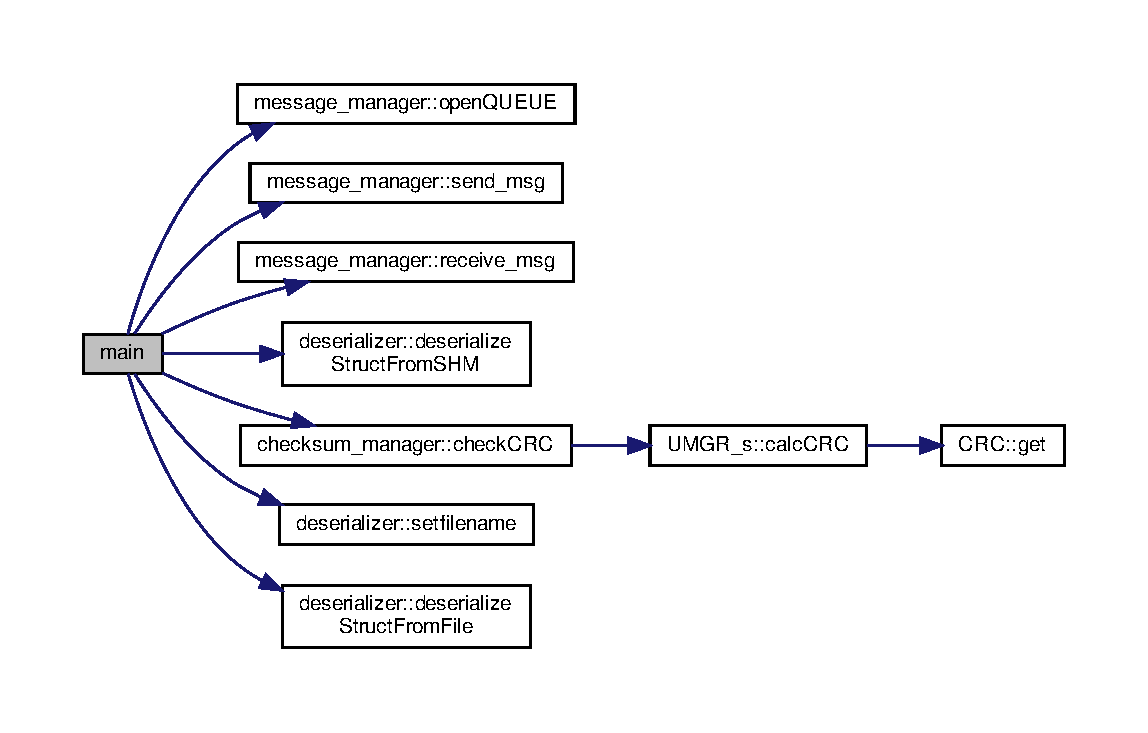
\includegraphics[width=350pt]{main_8cpp_a3c04138a5bfe5d72780bb7e82a18e627_cgraph}
\end{center}
\end{figure}

\hypertarget{message__manager_8cpp}{}\section{/home/visxim/\+C\+Lion\+Projects/\+Adaptive\+Dummy\+Process/message\+\_\+manager.cpp File Reference}
\label{message__manager_8cpp}\index{/home/visxim/\+C\+Lion\+Projects/\+Adaptive\+Dummy\+Process/message\+\_\+manager.\+cpp@{/home/visxim/\+C\+Lion\+Projects/\+Adaptive\+Dummy\+Process/message\+\_\+manager.\+cpp}}


Message\+\_\+manager for managing the synchronization between processes.  


{\ttfamily \#include \char`\"{}message\+\_\+manager.\+h\char`\"{}}\newline
Include dependency graph for message\+\_\+manager.\+cpp\+:
\nopagebreak
\begin{figure}[H]
\begin{center}
\leavevmode
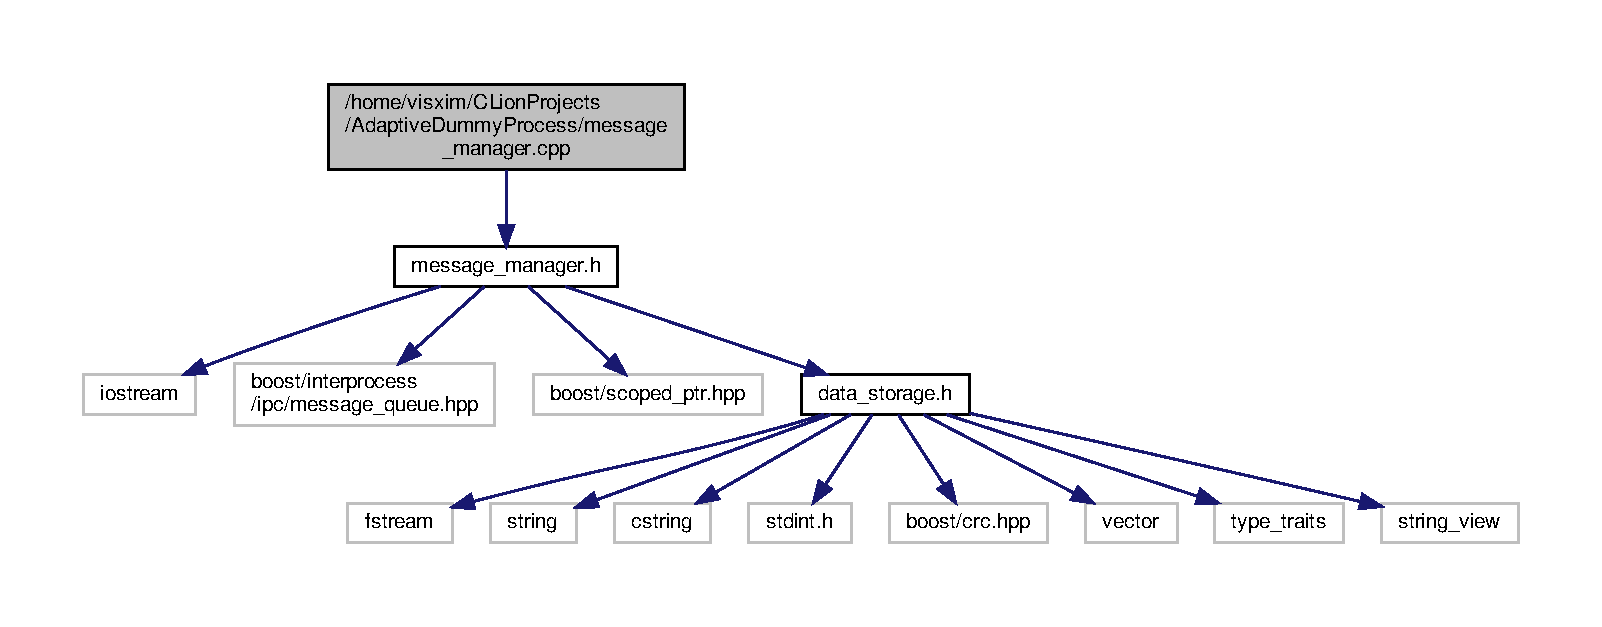
\includegraphics[width=350pt]{message__manager_8cpp__incl}
\end{center}
\end{figure}


\subsection{Detailed Description}
Message\+\_\+manager for managing the synchronization between processes. 

The Message\+\_\+manager managed all synchronization between processes via message queue 
\hypertarget{shared__memory_8cpp}{}\section{/home/visxim/\+C\+Lion\+Projects/\+Adaptive\+Dummy\+Process/shared\+\_\+memory.cpp File Reference}
\label{shared__memory_8cpp}\index{/home/visxim/\+C\+Lion\+Projects/\+Adaptive\+Dummy\+Process/shared\+\_\+memory.\+cpp@{/home/visxim/\+C\+Lion\+Projects/\+Adaptive\+Dummy\+Process/shared\+\_\+memory.\+cpp}}
{\ttfamily \#include \char`\"{}shared\+\_\+memory.\+h\char`\"{}}\newline
Include dependency graph for shared\+\_\+memory.\+cpp\+:
\nopagebreak
\begin{figure}[H]
\begin{center}
\leavevmode
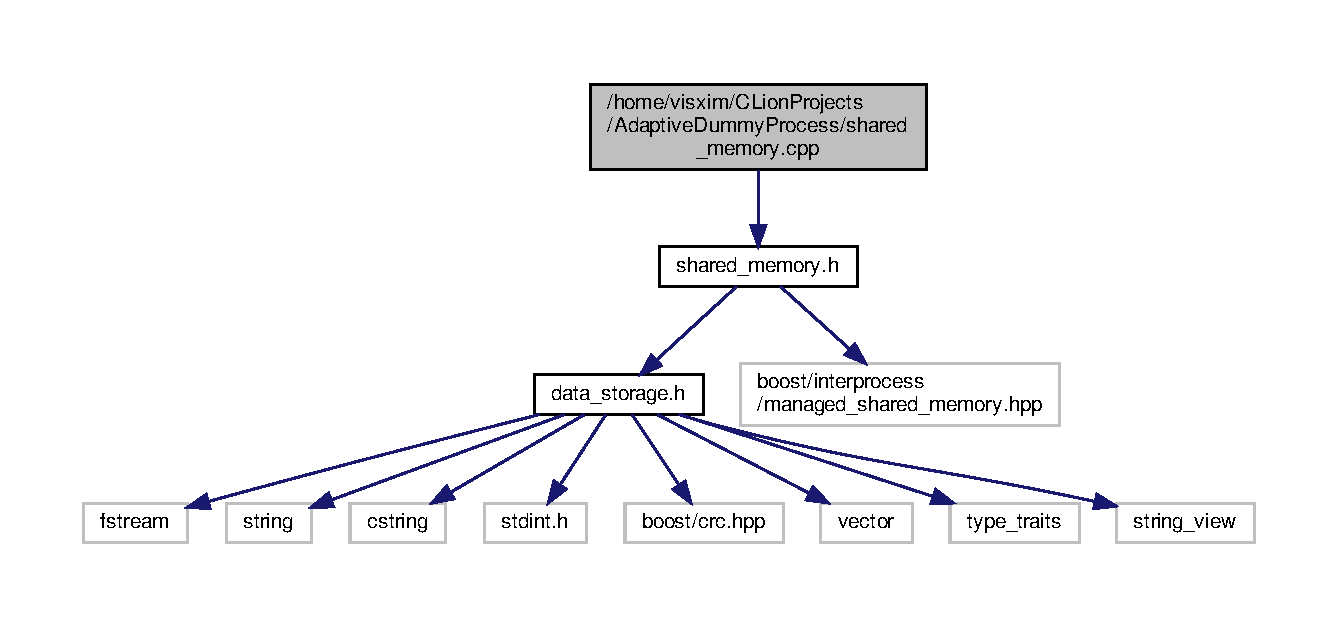
\includegraphics[width=350pt]{shared__memory_8cpp__incl}
\end{center}
\end{figure}

\hypertarget{time-tp_8cpp}{}\section{/home/visxim/\+C\+Lion\+Projects/\+Adaptive\+Dummy\+Process/time-\/tp.cpp File Reference}
\label{time-tp_8cpp}\index{/home/visxim/\+C\+Lion\+Projects/\+Adaptive\+Dummy\+Process/time-\/tp.\+cpp@{/home/visxim/\+C\+Lion\+Projects/\+Adaptive\+Dummy\+Process/time-\/tp.\+cpp}}
{\ttfamily \#include \char`\"{}time-\/tp.\+h\char`\"{}}\newline
Include dependency graph for time-\/tp.cpp\+:
\nopagebreak
\begin{figure}[H]
\begin{center}
\leavevmode
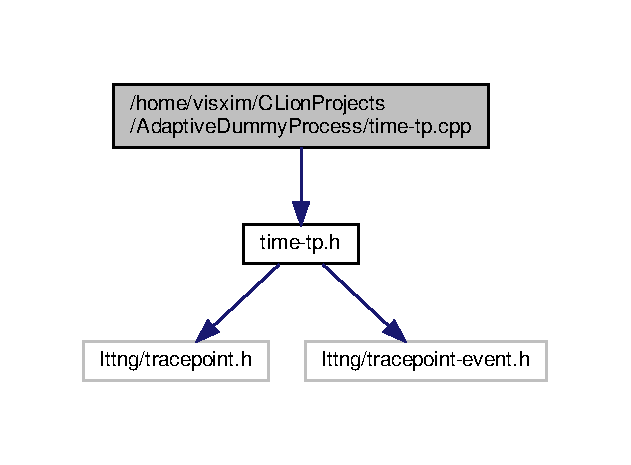
\includegraphics[width=303pt]{time-tp_8cpp__incl}
\end{center}
\end{figure}
\subsection*{Macros}
\begin{DoxyCompactItemize}
\item 
\#define \hyperlink{time-tp_8cpp_aeb980b4a64d9b54d660780a30415b0bc}{T\+R\+A\+C\+E\+P\+O\+I\+N\+T\+\_\+\+C\+R\+E\+A\+T\+E\+\_\+\+P\+R\+O\+B\+ES}
\item 
\#define \hyperlink{time-tp_8cpp_a71ad37c54f22eb10bdfed4267d53bd79}{T\+R\+A\+C\+E\+P\+O\+I\+N\+T\+\_\+\+D\+E\+F\+I\+NE}
\end{DoxyCompactItemize}


\subsection{Macro Definition Documentation}
\mbox{\Hypertarget{time-tp_8cpp_aeb980b4a64d9b54d660780a30415b0bc}\label{time-tp_8cpp_aeb980b4a64d9b54d660780a30415b0bc}} 
\index{time-\/tp.\+cpp@{time-\/tp.\+cpp}!T\+R\+A\+C\+E\+P\+O\+I\+N\+T\+\_\+\+C\+R\+E\+A\+T\+E\+\_\+\+P\+R\+O\+B\+ES@{T\+R\+A\+C\+E\+P\+O\+I\+N\+T\+\_\+\+C\+R\+E\+A\+T\+E\+\_\+\+P\+R\+O\+B\+ES}}
\index{T\+R\+A\+C\+E\+P\+O\+I\+N\+T\+\_\+\+C\+R\+E\+A\+T\+E\+\_\+\+P\+R\+O\+B\+ES@{T\+R\+A\+C\+E\+P\+O\+I\+N\+T\+\_\+\+C\+R\+E\+A\+T\+E\+\_\+\+P\+R\+O\+B\+ES}!time-\/tp.\+cpp@{time-\/tp.\+cpp}}
\subsubsection{\texorpdfstring{T\+R\+A\+C\+E\+P\+O\+I\+N\+T\+\_\+\+C\+R\+E\+A\+T\+E\+\_\+\+P\+R\+O\+B\+ES}{TRACEPOINT\_CREATE\_PROBES}}
{\footnotesize\ttfamily \#define T\+R\+A\+C\+E\+P\+O\+I\+N\+T\+\_\+\+C\+R\+E\+A\+T\+E\+\_\+\+P\+R\+O\+B\+ES}

\mbox{\Hypertarget{time-tp_8cpp_a71ad37c54f22eb10bdfed4267d53bd79}\label{time-tp_8cpp_a71ad37c54f22eb10bdfed4267d53bd79}} 
\index{time-\/tp.\+cpp@{time-\/tp.\+cpp}!T\+R\+A\+C\+E\+P\+O\+I\+N\+T\+\_\+\+D\+E\+F\+I\+NE@{T\+R\+A\+C\+E\+P\+O\+I\+N\+T\+\_\+\+D\+E\+F\+I\+NE}}
\index{T\+R\+A\+C\+E\+P\+O\+I\+N\+T\+\_\+\+D\+E\+F\+I\+NE@{T\+R\+A\+C\+E\+P\+O\+I\+N\+T\+\_\+\+D\+E\+F\+I\+NE}!time-\/tp.\+cpp@{time-\/tp.\+cpp}}
\subsubsection{\texorpdfstring{T\+R\+A\+C\+E\+P\+O\+I\+N\+T\+\_\+\+D\+E\+F\+I\+NE}{TRACEPOINT\_DEFINE}}
{\footnotesize\ttfamily \#define T\+R\+A\+C\+E\+P\+O\+I\+N\+T\+\_\+\+D\+E\+F\+I\+NE}


%--- End generated contents ---

% Index
\backmatter
\newpage
\phantomsection
\clearemptydoublepage
\addcontentsline{toc}{chapter}{Index}
\printindex

\end{document}
